\documentclass[12pt, a4paper, bibliography=totoc]{scrartcl}

% personal data
\date{\today}


% language
\usepackage{polyglossia}
\setmainlanguage{english}
\setotherlanguages{german}
\usepackage{microtype}
\usepackage{dcolumn}

\usepackage[style=numeric,
			natbib=true,
			backend=biber]{biblatex}		%Bibliographie
\usepackage[autostyle=true,
			 german=quotes]
			 {csquotes}					%Anführungszeichen
\usepackage{blindtext}


%math and theorems
\usepackage{amsmath}
\usepackage{amssymb}
\usepackage{amsopn}					%Matheoperatoren
\usepackage[amsmath,thmmarks,hyperref]{ntheorem}
\usepackage{mathtools}
\usepackage{mathdots}					%Punkte
\usepackage{dsfont}
\usepackage{upgreek}					%Griechische Buchstaben
\usepackage{bbm}						%Mengensymbol
\usepackage{physics}					%Physiksymbole
\usepackage{relsize}						%Größenangaben
\usepackage[separate-uncertainty,
			per-mode=symbol]
			{siunitx}					%Einheiten
%\usepackage{tikz}						%Zeichnen
\usepackage{upgreek}					%Griechische Buchstaben
\usepackage{enumitem}
\setlist{nolistsep}


%useful packages
%\usepackage{geometry}
\usepackage{xcolor}
\usepackage{graphicx}
\usepackage{float}
\usepackage{csquotes}
\usepackage{todonotes}
\usepackage{booktabs}
\usepackage{array}
\usepackage[labelfont=bf]{caption}
\usepackage{wrapfig}
\usepackage{enumitem}
%\usepackage{xr} % cross referencing
%\usepackage{titling}
%\usepackage{titlesec}
%\usepackage[Bjornstrup]
%			{fncychap}					%Kapitellayout


\setmainfont{Linux Libertine O}
\setsansfont{Linux Biolinum O}

\usepackage{scrhack}					%Verbesserung Pakete
\usepackage{xltxtra}						%fontec


\newcommand{\im}{\mathrm{i}}
\newcommand{\e}{\mathrm{e}}
\renewcommand{\pi}{\uppi}
\renewcommand{\epsilon}{\varepsilon}


\addbibresource{bibliography.bib}

%color settings
\definecolor{myred}{RGB}{196,19,47} 
\definecolor{myblue}{RGB}{0,139,139}


%appendix
\usepackage[toc,page]{appendix}

%killing indent
\setlength{\parindent}{0pt}
\usepackage{multicol}
\usepackage{siunitx}
\usepackage{hyperref}


\title{FP18 Atmospheric Trace Gases}
\author{Aaron Mielke \& Thomas Ackermann}
\date{\today}

\begin{document}

\begin{center}
	\makeatletter
	\thispagestyle{empty}
	\large{Fortgeschrittenen-Praktikum}	
	\hfill
    \large{Summer term 2019}
    \vspace{5mm}
	\rule{\textwidth}{0.2pt}
    \vfill
	\Huge\textbf{\@title} \\
	\vspace{10mm}
	\large{\@author} \\
	\normalfont
	\vfill	
	\makeatother
\end{center}

\normalsize

\section*{Abstract}

This experiment was conducted in the scope of the advanced lab course in physics at the University of Heidelberg. \\
The main goal was to find the concentration of \ch{NO2} and \ch{O3} in the atmosphere by using the DOAS method. \\
Measurements were taken in the week of the $29^\text{th}$ april, 2019.
Due to a lack of clear sky conditions during this week, the analyzed data was from the $23^\text{th}$ april, 2019. 
One calculated a vertical column density of $\sim 300 \si{DU}$ for \ch{O3}, which is an underestimation when compared with the data NASA provided (measured $\sim 350 \si{DU}$).\\ 
The measurements of the tropospheric concentrations was not very descriptively because heavy and thick clouds interfered with the measurements. 
Regardless of this setback one found at least a trend for the three trace gases \ch{O3}, \ch{No2} and \ch{O4}. 
The ratio between the measurments at $7^{\circ}$ and $12^{\circ}$ yields that \ch{O3} is mainly found in the staratosphere where the other two are present in the troposhere aswell.

\newpage

\tableofcontents
\newpage

\begin{multicols}{2}

\section{Theoretische Grundlagen}\label{sec:Intro}
Die genaue Bestimmung der Konzentration verschiedener Spurengase ist eine wichtige Aufgabe in der Umweltphysik.
    Eine Möglichkeit zur Bestimmung ist das Prinzip der \textit{Differential Optical Absorption Spectrocopy } (DOAS), welche zahlreiche Anwendungen findet.
Einige Grundlagen zur Atmosphäre und die Funktionsweise von DOAS sollen im Folgenden erklärt werden.

\subsection{Zusammensetzung der Atmosphäre}\label{ssec:Comp_Atmo}

Die Atmosphäre der Erde besteht aus einer Mischung verschiedener Gase.
Tabelle \ref{fig:atm_comp} zeigt eine Liste der Hauptkomponenten.

\begin{center}

\begin{tabular*}{\linewidth}{@{\extracolsep{\fill}}  c c c}
	\toprule
	Gas & Symbol & Rel. Anteil \\
	\midrule
	Stickstoff & \ch{N2} & $78.084 \%$ \\
    Sauerstoff & \ch{O2} & $20.942\%$ \\
    Argon & \ch{Ar} & 0.934 \% \\
    Wasserdampf & \ch{H2O} & ca. 1 \% \\
    Kohlenstoffdioxid & \ch{CO2} & 358 \si{ppmv} \\
    Neon & \ch{Ne} & 18.2 \si{ppmv} \\
    Methan & \ch{CH4} & 1.75 \si{ppmv} \\
    Wasserstoff & \ch{H2} & 0.55 \si{ppmv} \\
    Kohlenmonoxid & \ch{CO} & 0.11 \si{ppmv} \\
    Ozon & \ch{O3} & 0.04 \si{ppmv} \\
	\bottomrule
\end{tabular*}
    \captionof{table}{Gase in der Atmosphäre \cite{atm_script}} %\cite{atm_components}
    \label{fig:atm_comp}
\end{center}

Ozon ist ein sehr effizienter Absorber von UV Strahlung und bietet daher einen Schutz vor schädlicher Strahlung für den Menschen.\\
    Die Atmosphäre lässt sich in verschiedene Zonen unterscheiden (siehe Abbildung \ref{fig:atmosphere}).
In diesem Versuch werden allerdings nur die Tropo- und Stratosphäre untersucht.


\begin{center}
    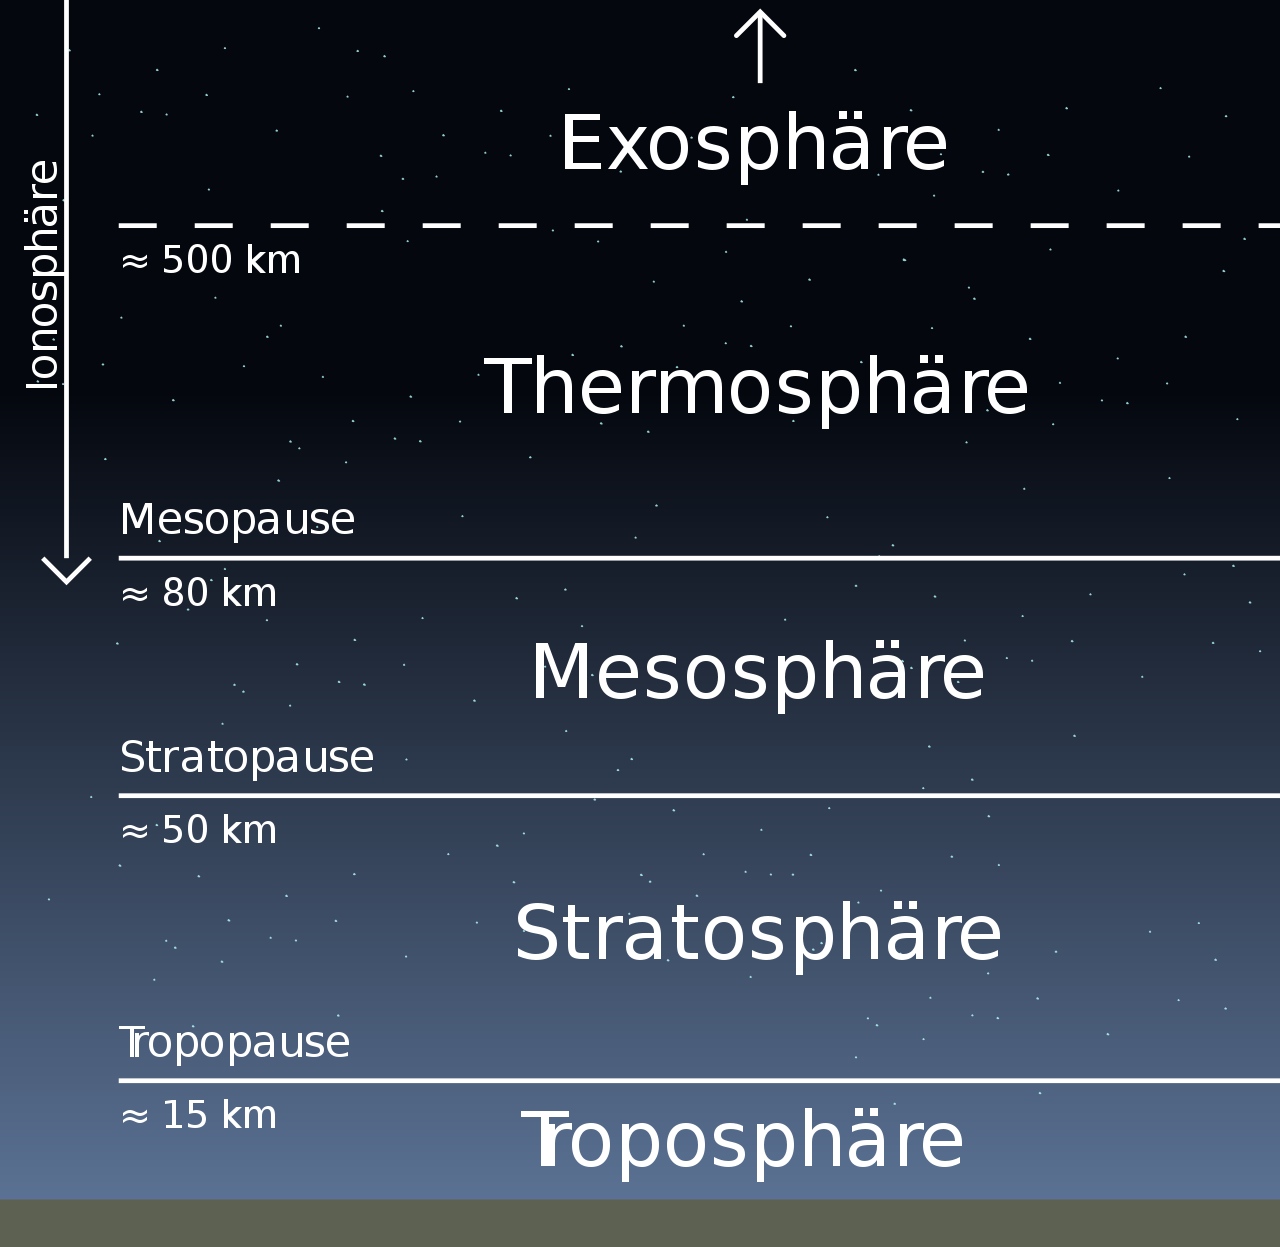
\includegraphics[width=.8\linewidth]{fig/erdatmosphäre.png}
    \label{fig:atmosphere}
   
    \captionof{figure}{Atmosphärische Schichten \footnotemark}

    \footnotetext{\url{https://upload.wikimedia.org/wikipedia/commons/4/47/Atmosphäre_Stufen.svg}}
\end{center}

\subsection{Messgrößen}\label{ssec:Messgröße}

Die Konzentration eines Spurengases ist die Zahl der Moleküle pro Volumeneinheit und hat daher die Dimension $\si{[Moleküle/cm^3]}$.\\
Eine andere wichtige Größe ist das Mischverhältnis.
Sie gibt den relative Anteil eines Spurengases im Vergleich zur Luftmenge an und wird mit \si{[ppm]} oder \si{[ppt]} angegeben. 
    Bei diesem Versuch ist ebenfalls die \textit{column density}
    \begin{align}
        \text{CD} = \int \rho(s) \dd s,
    \end{align}
    von großer Bedeutung, welche die Einheit $\si{[Moleküle / cm^2]}$ besitzt.
\subsection{DOAS}\label{ssec:DOAS}

\textit{Differential Optical Absorption Spectroscopy} (DOAS) wird verwendet um die Konzentration eines bestimmten Spurengases in der Atmosphäre zu bestimmen - was das Ziel dieses Experimentes ist.
Das Hauptprinzip ist das Folgende: 
    Man nimmt zwei Spektren auf, eines welches auf der Erde aufgenommen wurde (also mit Absorption des Sonnenlichtes durch die Atmosphäre) und eines bei dem die Atmosphäre nicht präsent ist (von Satelliten aus aufgenommen).
Jedes Gas absorbiert bestimmte Wellenlängen des Sonnenlichts.

\begin{center}
    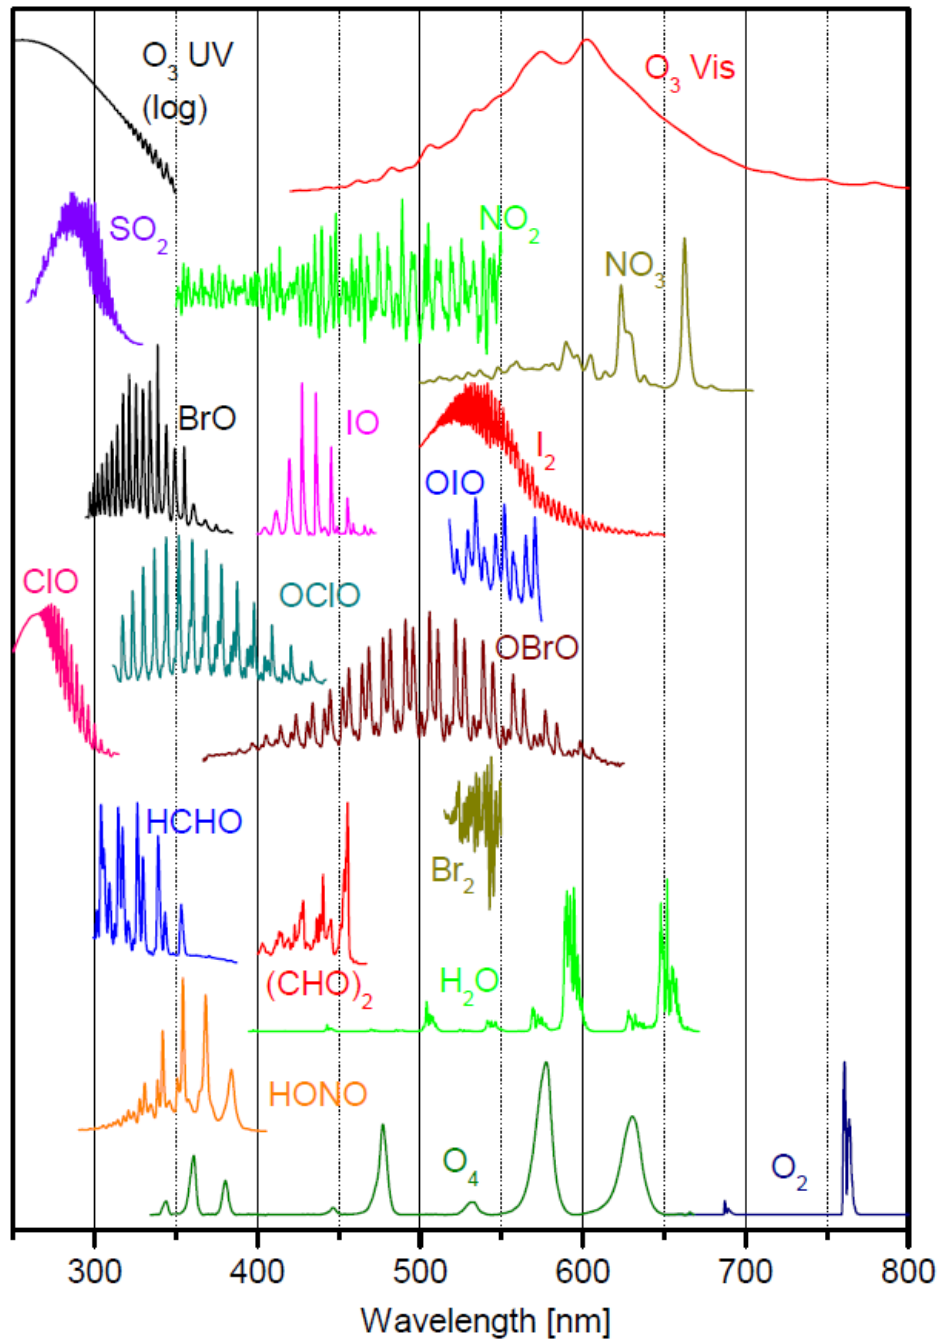
\includegraphics[width=0.7\linewidth]{fig/gas_spectra.png}
    \captionof{figure}{Charakteristische Linien verschiedener Gase \cite{atm_script}}	
    \label{fig:gas_spectra}
\end{center}

Wenn nun zwei Spektren, wie beschrieben, aufgenommen werden, 
kann das charakteristische Verhalten der Gase daran erkannt werden, dass die Intensitäten an manchen stellen kleiner sind.

Wenn man nun weiß welche Charakteristika zu welchen Gasen gehören kann die Dichte des Gases in der Atmosphäre bestimmt werden.\\
In diesem Versuchsaufbau steht allerdings kein Satellit zur Verfügung, so dass sich die Frage stellt wie man an ein Sonnenspektrum ohne atmosphärische Einwirkung erhält.

Die Lösung hier besteht daraus das Spektrum bei verschiedenen Sonnenzenitwinkeln oder Telesekopwinkeln aufzunehmen und dann zu vergleichen.
Die mittlere Weglänge die das Licht zurücklegt ist statistisch viel kürzer, wenn genau im Zenit gemessen wird als bei anderen Winkeln.
Daher ist hier die Absorption durch Spurengase viel geringer sodass man einen ähnlichen Unterschied wie bei einem Satelliten erhält.

\subsubsection{Lambert-Beer Gesetz}\label{sssec:Lamb-Beer_law}

Die Intensität eines Lichtstrahls (einer Elektromagnetischen Welle) nimmt durch Streuung und Absorption ab, wenn es durch Materie propagiert (siehe Abbildung \ref{fig:lambert-beer}).

\begin{center}
    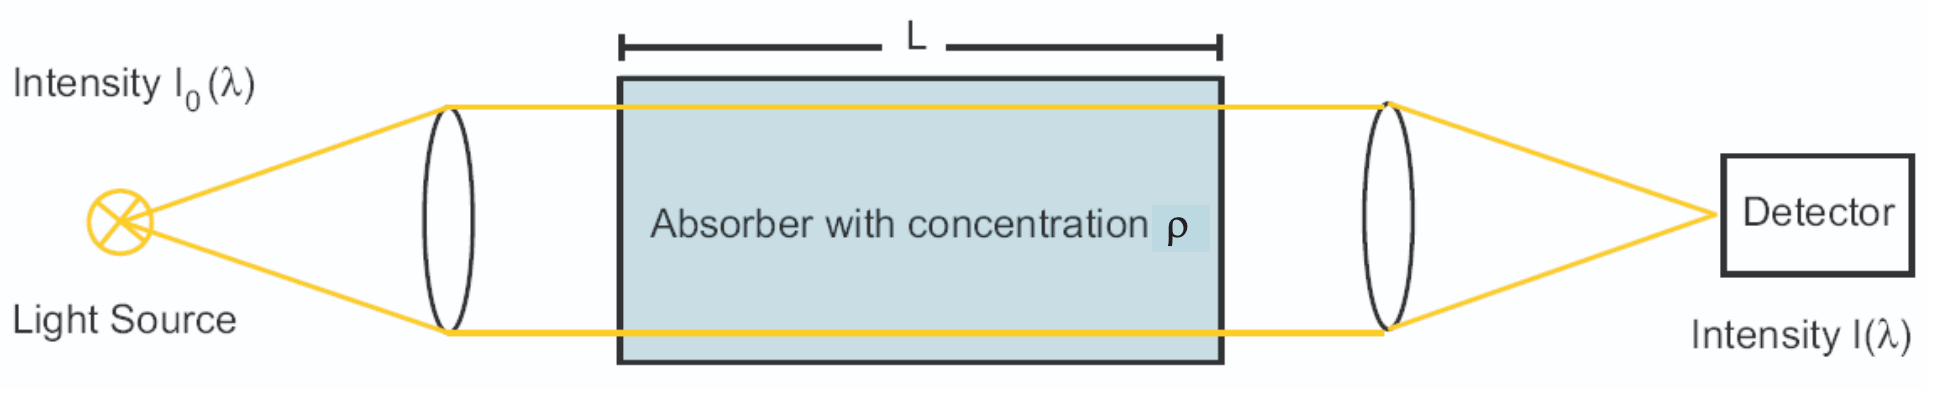
\includegraphics[width=\linewidth]{fig/lambert_beer.png}
    \captionof{figure}{Darstellung des Lambert-Beer Gesetzes \cite{atm_script}}
	\label{fig:lambert-beer}
\end{center}

Die Größe des Verlustes kann mithilfe des Lambert-Beer Gesetzes bestimmt werden.
Sei $I_0 (\lambda)$ die Startintensität des Lichtstrahls, dann ist die Intensität $I(\lambda, L)$ nachdem der Lichtstrahl eine Länge $L$ der Mediums überwunden hat
    
\begin{align}
    I(\lambda, L) = I_0 (\lambda) \exp \left( - \rho L \sigma (\lambda)\right) ,\label{eq:lambert_beer_law}
\end{align}

wobei $\sigma (\lambda)$ der Absorptionswirkungsquerschnitt und $\rho$ die Konzentration des Spurengases ist.
Der Absorptionswirkungsquerschnitt gibt eine Wahrscheinlichkeit für eine Absorption bei einer bestimmten Wellenlänge $\lambda$ an.

\subsection{Kurzband Komponenten}\label{ssec:Kurzband}

\subsubsection{Fraunhofer Referenzspektrum}\label{sssec:fraunhofer_reference}

Das Fraunhoferspektrum \ref{fig:fraunhofer_spectrum} zeigt das unbeeinflusste Spektrum des Sonnenlichtes. 
Dieses zeigt viele Strukturen, die in DOAS berücksichtigt werden müssen. 
Daher wird ein Fraunhofer Referenzspektrum verwendet.

\begin{center}
    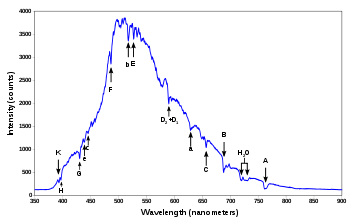
\includegraphics[width=\linewidth]{fig/fraunhofer_linien.png}
    \captionof{figure}{Fraunhofer Spektrum \footnotemark}	
    \footnotetext{\url{https://en.wikipedia.org/wiki/Fraunhofer_lines#/media/File:Spectrum_of_blue_sky.svg}}
    \label{fig:fraunhofer_spectrum}
\end{center}



\subsubsection{Spurengas Absorption}\label{sssec:trace_gas_absorption}

Die Hauptmessgröße des DOAS ist die \textit{slant column density} (SCD oder $S$),
welche als die integrierte Dichte eines Spurengases $i$ entlang eines Lichtpfades der Länge $L$ definiert ist.
    
\begin{align}
    \text{SCD} = S_i (\lambda) = \int_0^{L(\lambda)} \rho_i (s) \dd s ,\label{eq:SCD}
\end{align}

\subsubsection{Ring-Effekt}

Wie in Abbildung \ref{fig:fraunhofer_spectrum} zu sehen gibt es im Fraunhoferspektrum verschiedene Absorptionslinien.
Es ist zu beobachten, dass die Tiefe dieser Linien schwächer ist, wenn man gestreutes Sonnenlicht mit direktem Sonnenlicht vergleicht.\\
Der Grund dafür ist inelastische Raman-Streuung, welche dazu führt, dass die Wellenlängen der Photonen während der Streuung verändert werden.
Durch Änderung der Wellenlängen werden die Absorptionslinien aufgefüllt,
dies bezeichnet man als \textit{Ring-Effekt}.

\subsection{Breitband Komponenten}

Das Sonnenlicht wird von Aerosolen und Wassertröpfchen in den Wolken gestreut und absorbiert (\textit{Mie Streuung}),sowie von Luftmolekülen gestreut (\textit{Rayleigh Streuung}).
Die Summe aus Streuungs- und Absorptionseffekten wird als Extinktion ($\epsilon_M$ und $\epsilon_R$ in diesem Fall) bezeichnet.
Beide Prozesse sind elastisch, was bedeutet, dass sich die Wellenlängen nicht verändern.
Die Wahrscheinlichkeit für Rayleigh Streuung skaliert mit $\lambda^{-4}$ und ist somit besonders bei kurzen Wellenlängen vorhanden.
Mie Streuung hängt im Gegensatz dazu nicht so stark von der Wellenlänge ab.

\begin{center}
    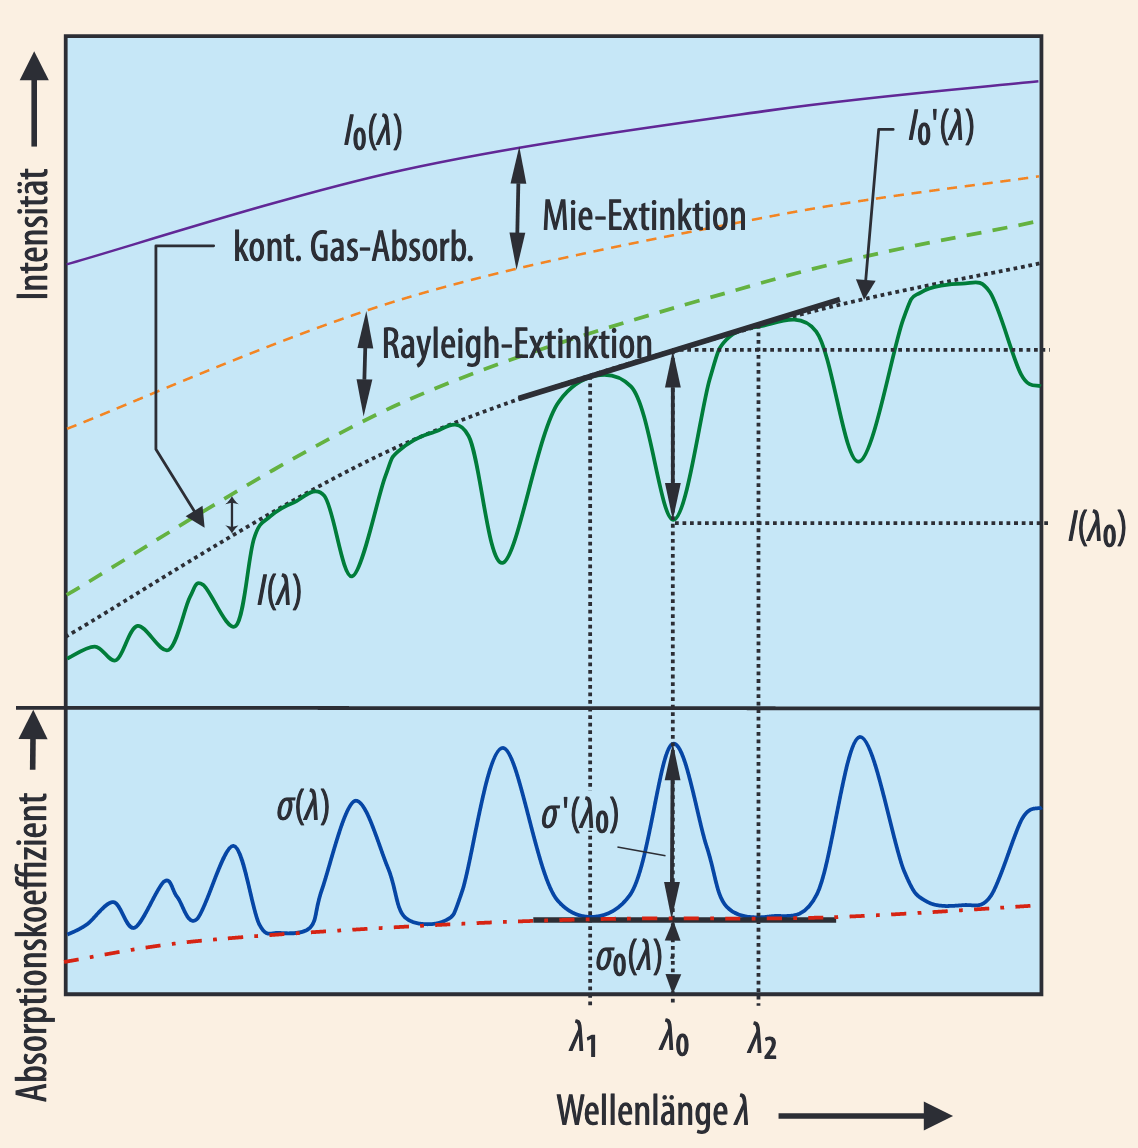
\includegraphics[width=0.8\linewidth]{fig/rayleigh_mie.png}
    \captionof{figure}{Darstellung Rayleigh- und Mie-Extinktion \cite{platt10}}	
    \label{fig:rayleigh_mie}
\end{center}



\subsection{Modifiziertes Lambert-Beer Gesetz}\label{ssec:mod_lamb-beer_law}

Wenn man nun diese Effekte mit einbezieht, so erhält man ein modifiziertes Lambert-Beer Gesetz.

\begin{align*}
    I(\lambda, L) = & I_0 (\lambda) \exp \left( -R - \sum_i \sigma_i
    S_i \right) \times \\
    & \exp \left[ - L \left( \sigma_{i0} \rho_o + \epsilon_R + \epsilon_M \right) \right], \label{eq:mod_lambert_beer_law}
\end{align*}

Die erste Exponentialfunktion beinhaltet alle Kurzbandeffekte und die zweite alle Breitbandeffekte.
Wenn man das modifizierte Lambert-Beer Gesetz nun nach $\log \frac{I}{I_0}$ umformt erhält man die optische Dichte $\tau$
\begin{align}
\tau &= \log \frac{I}{I_0} \\
    &= - R(\lambda) - \sum_i \sigma_i (\lambda) S_i (\lambda) - \sum_k b_k \lambda^k.\label{eq:optical_density}
\end{align}

Hierbei berücksichtigt das Polynom $\sum b_k \lambda^k$ Breitbandeffekte und $R(\lambda)$ ist das Ring-Spektrum.\\
Bei DOAS werden nun alle besprochenen Effekte miteinbezogen und ein Modell für die optische Dichte erstellt. 
Das Modell wird dann mit der gemessenen optischen Dichte verglichen und ein Fit erzeugt, welcher entsteht indem die Parameter so variiert werden, dass 

\begin{align*}
    \chi^2 = ( \log \frac{I_0 + I_\text{ofs}}{I} - R & - \sum_i \sigma_i S_i \\ 
    & - \sum_k b_k \lambda^k )^2 ,
\end{align*}

minimiert wird. Durch $I_{ofs}$ kann das, falls es zu ungewollten Streuungen im Spektrometer kommt, \textit{Streulicht} berücksichtigt werden. Dies ist vor allem dann anzuwenden, falls die Streulichtintensität über das Spektrum variiert und somit die optische Dichte beeinflussen kann.  

\section{Versuchsdurchführung}\label{sec:versuchsdurchführung}

\subsection{Software kennenlernen}\label{get_to_know_the_software}

Während des Versuches wurde das Programm \verb*+DOASIS+ verwendet um die Spektren aufzunehmen und später die Fits durchzuführen.\\
Zu Beginn wurde durch variieren der Messzeit (\textit{exposure time}) und der Anzahl der Scans (\textit{exposures}) ein erster Überblick über das Programm \verb*+DOASIS+ verschafft.

\begin{center}
	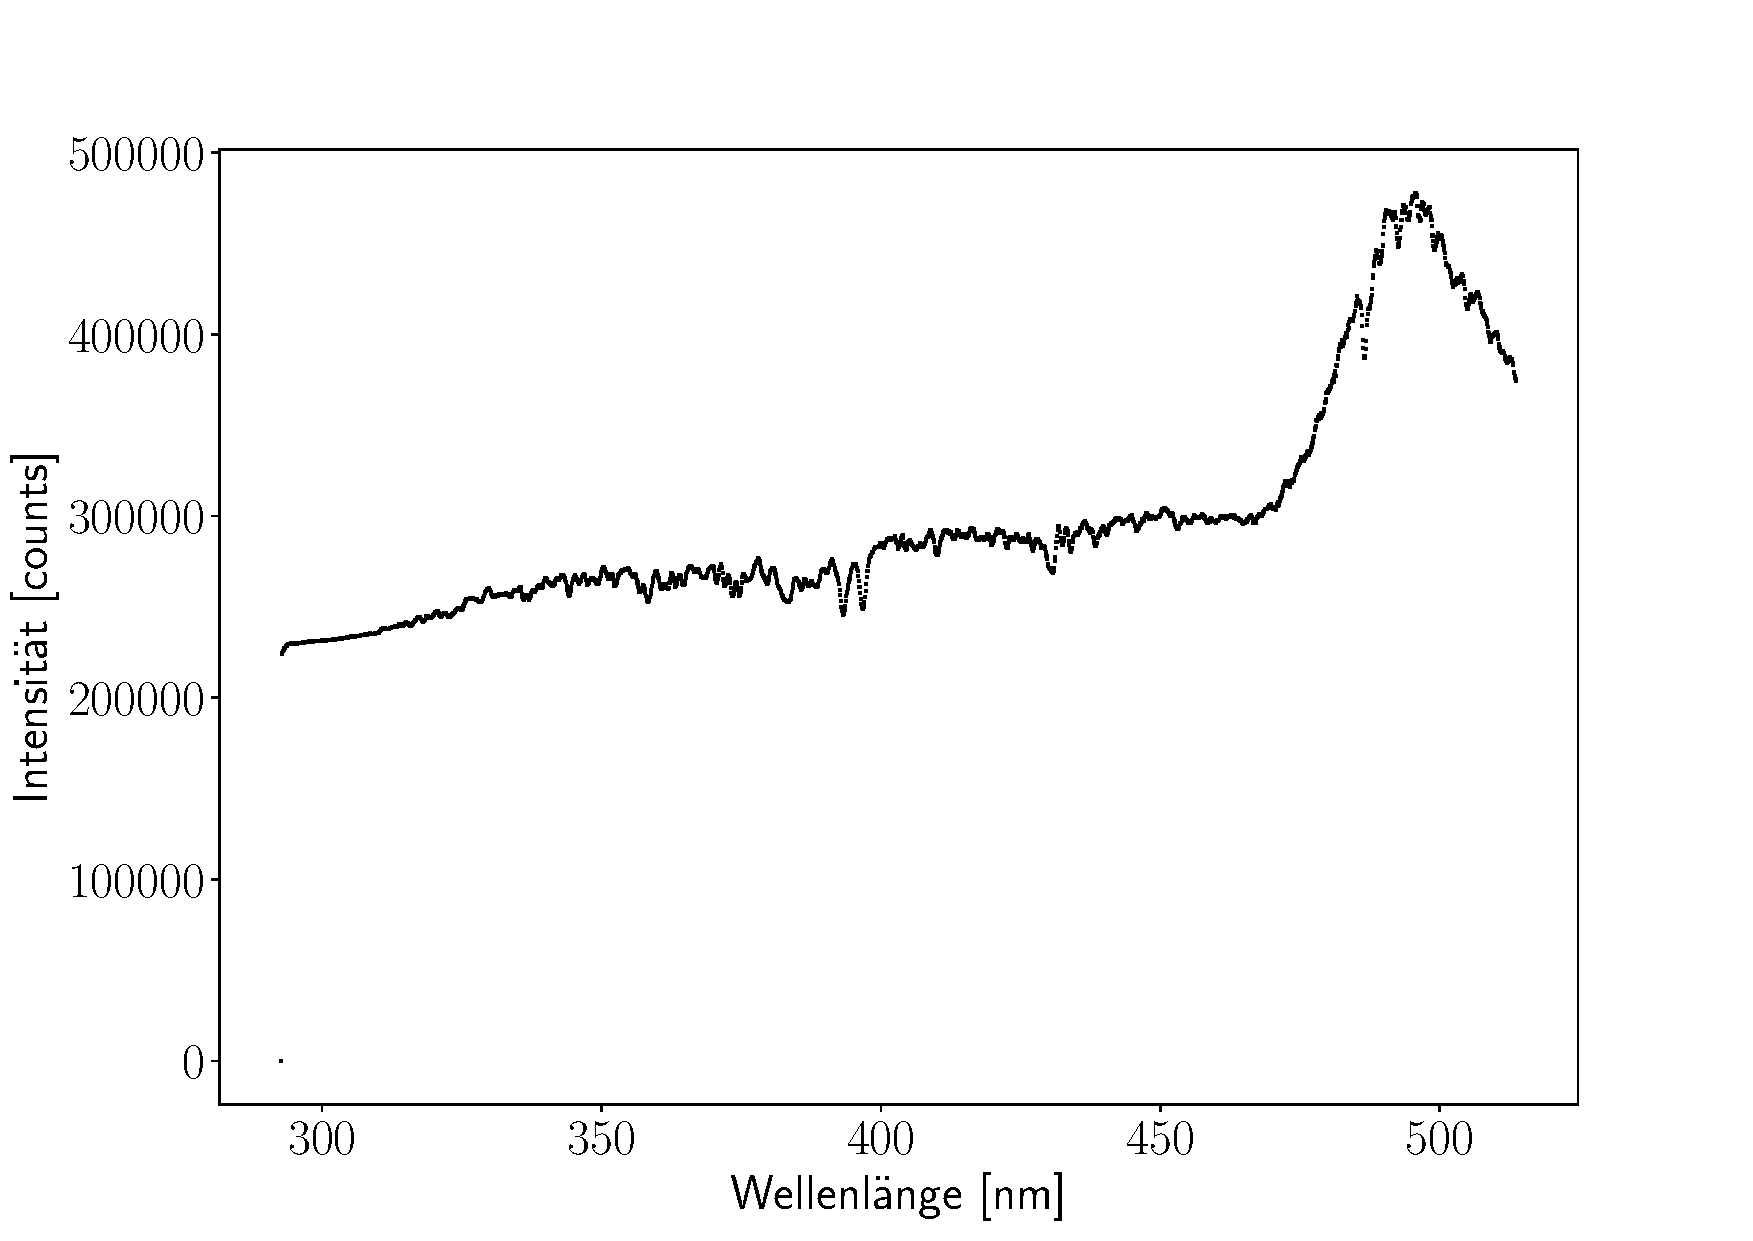
\includegraphics[width=\linewidth]{fig/test_spektrum.pdf}
    \captionof{figure}{Testspektrum einer Halogenlampe}
	\label{fig:test_spectrum}

\end{center}

\subsection{Charakterisierung der Messinstrumente}\label{ssec:characteristic_of_the_instruments}

\subsubsection{Offset und Dunkelstrom}\label{sssec:O&D}

Es gibt zwei Haupteffekte die Ungenauigkeiten bei der Messung verursachen können.
Durch Brownsche Bewegung in den Kabeln wird ein kleiner elektrischer Strom erzeugt, den man auch als Dunkelstrom bezeichnet.
Um die Größenordnung des Dunkelstromes einzuschätzen werden einminütige Messungen durchgeführt, bei denen die Kamera abgedeckt ist.\\
Die CCD-Kameras haben außerdem ein Offset, welcher durch viele kurze Messungen bestimmt werden kann.\\
Dunkelstrom und Offset müssen bei jedem folgenden Spektrum abgezogen werden.
Die Messung des Offsets wurde als erstes Durchgeführt. 
Hierbei wurden $20000$ Messungen mit jeweils $3$ \si{ms} Messzeit durchgeführt.
Anschließend wurde der Dunkelstrom bei verschiedenen Messzeiten gemessen (siehe Abbildung \ref{fig:dark_current}).
    
\begin{center}
	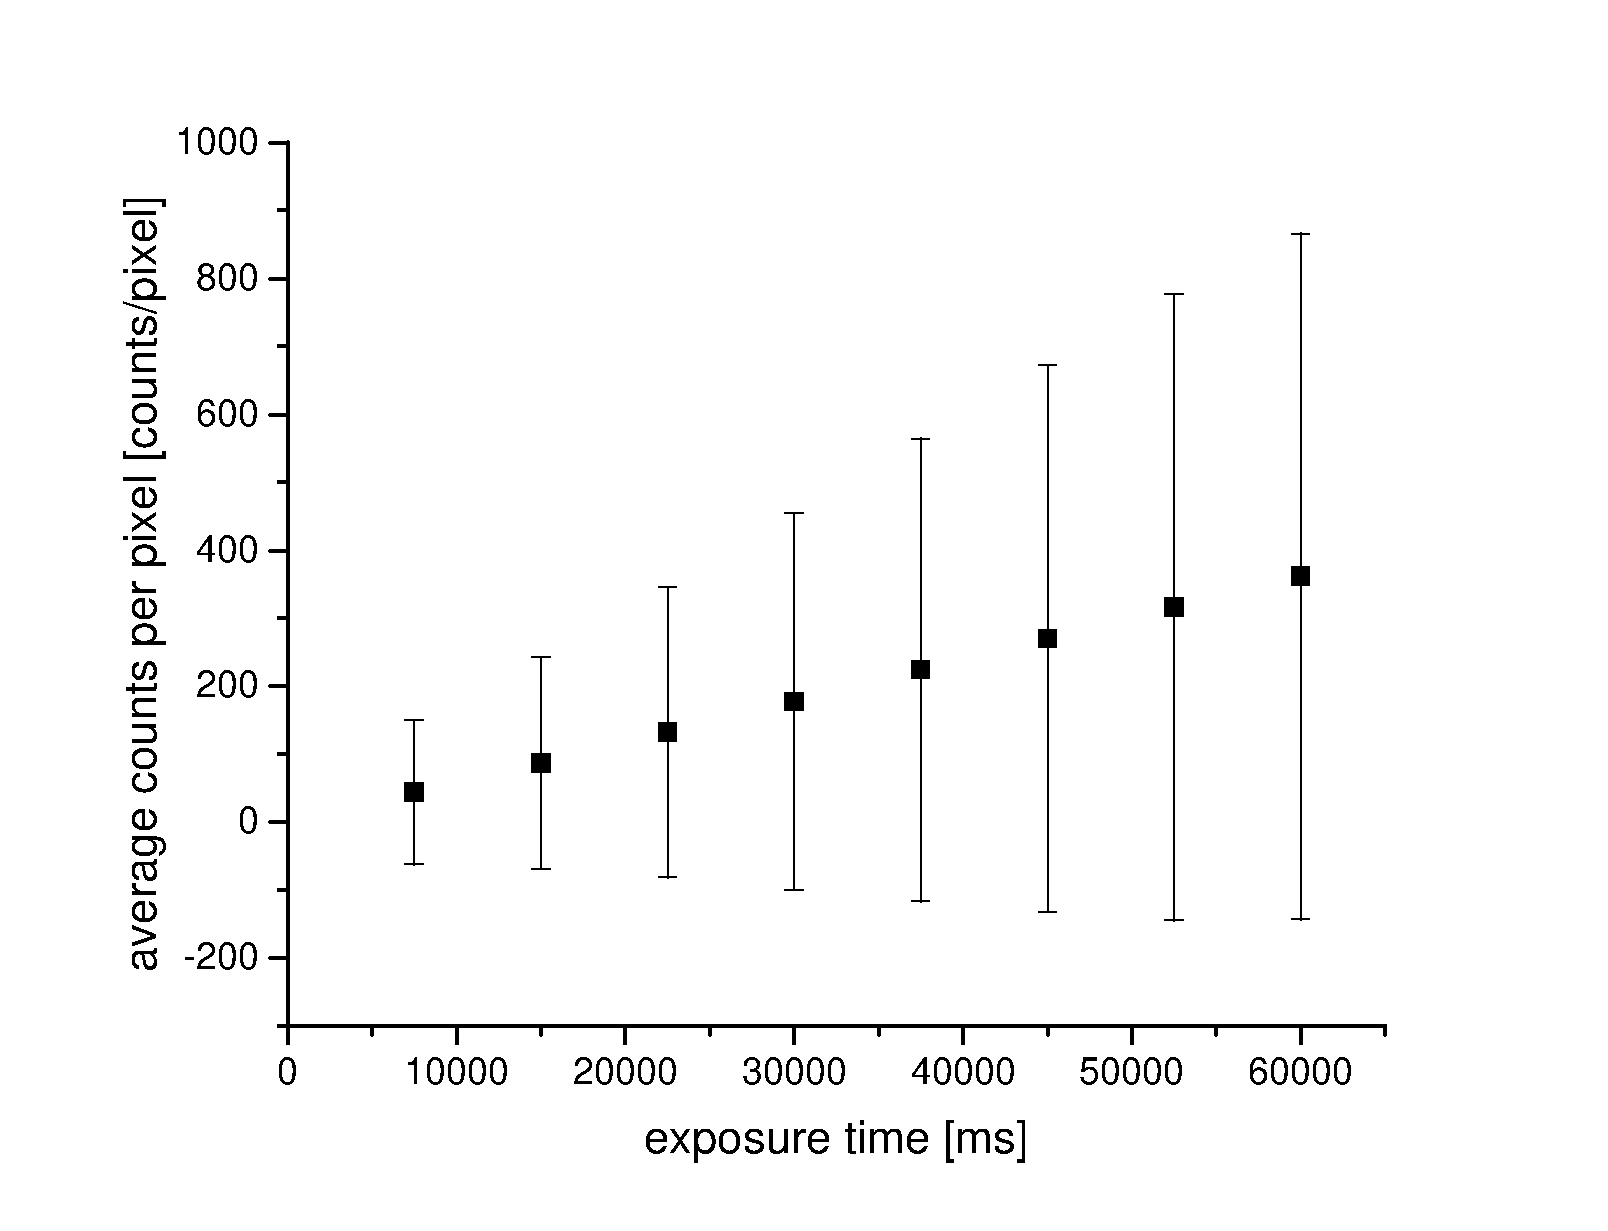
\includegraphics[width=\linewidth]{fig/dark_current_exposure_time_plot.pdf}
    \captionof{figure}{Abhängigkeit des Dunkelstromes von der Messzeit}
	\label{fig:dark_current}
\end{center}

\subsubsection{Instrumenten- und totales Rauschen}\label{sssec:instrumental_total_noise}

Wie im oberen Abschnitt \ref{sssec:O&D} gesehen, entstehen Messfehler, die zeitlich nicht konstant sind. Zunächst widmet man sich dem instrumentenbedingten Rauschen.
Dazu werden zwei Offsets mit identischen Einstellungen kurz hintereinander aufgenommen, über die entstandene Differenz ($\sigma_D$) lässt sich dann das Instrumentenrauschen bestimmen 

\begin{align}
\sigma_{I} = \frac{\sigma_D}{\sqrt{2}}.\label{eq:instrumental_noise}
\end{align}

Ein Auftragen des Rauschens gegen die Anzahl der Scans liefert einen linearen Zusammenhang (siehe Diagramm \ref{fig:instrumental_noise})

\begin{center}
	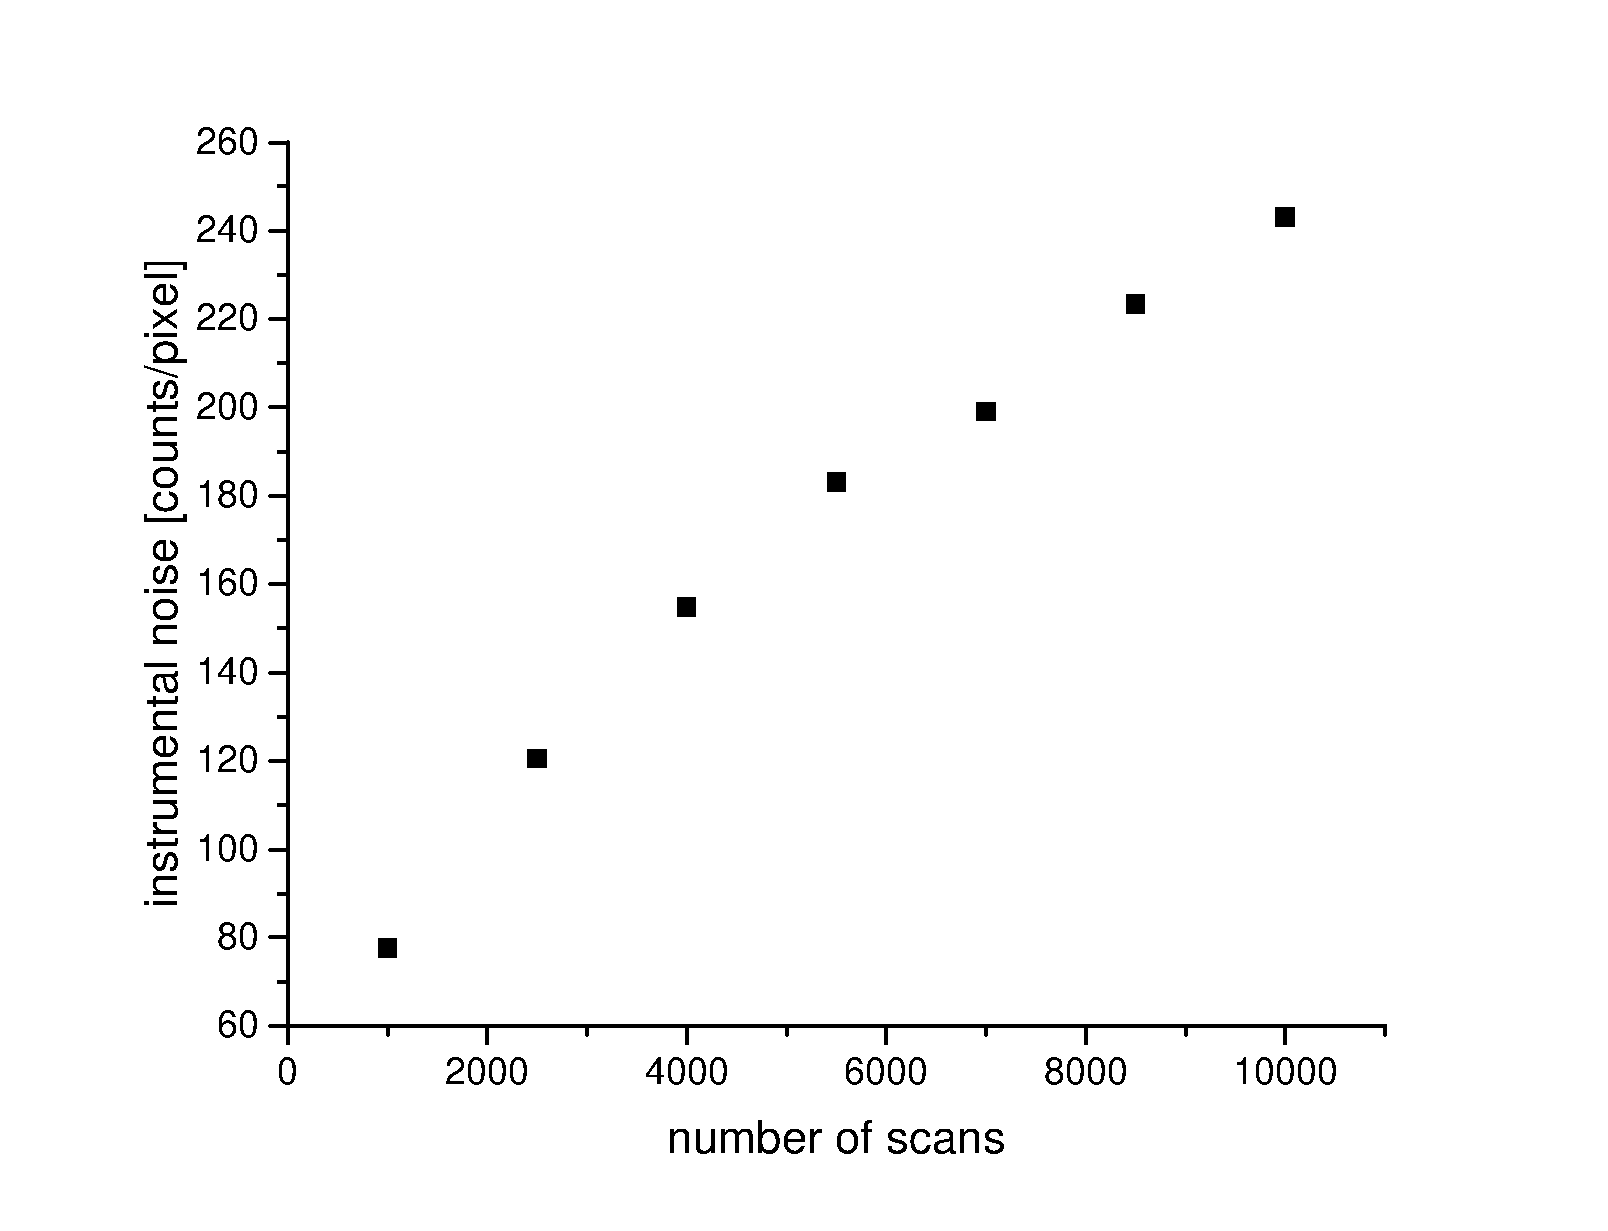
\includegraphics[width=\linewidth]{fig/instrumental_noise_diagramm.pdf}
	\captionof{figure}{Abhängigkeit des Instrumentenrauschens von der Anzahl der Scans}
	\label{fig:instrumental_noise}
\end{center}  

Zur Bestimmung des totalen Rauschens wurde nun das Spektrum einer Halogenlampe aufgenommen.
Es wurden ebenfalls wieder jeweils zwei Spektren bei identischen Einstellungen kurz hintereinander aufgenommen. 
Um systematische Strukturen, wie das Schwanken der Lampenintensität zwischen den beiden Messungen, zu berücksichtigen wurde ein Hochpassfilter an die Daten angelegt.
%\newpage
\begin{center}
	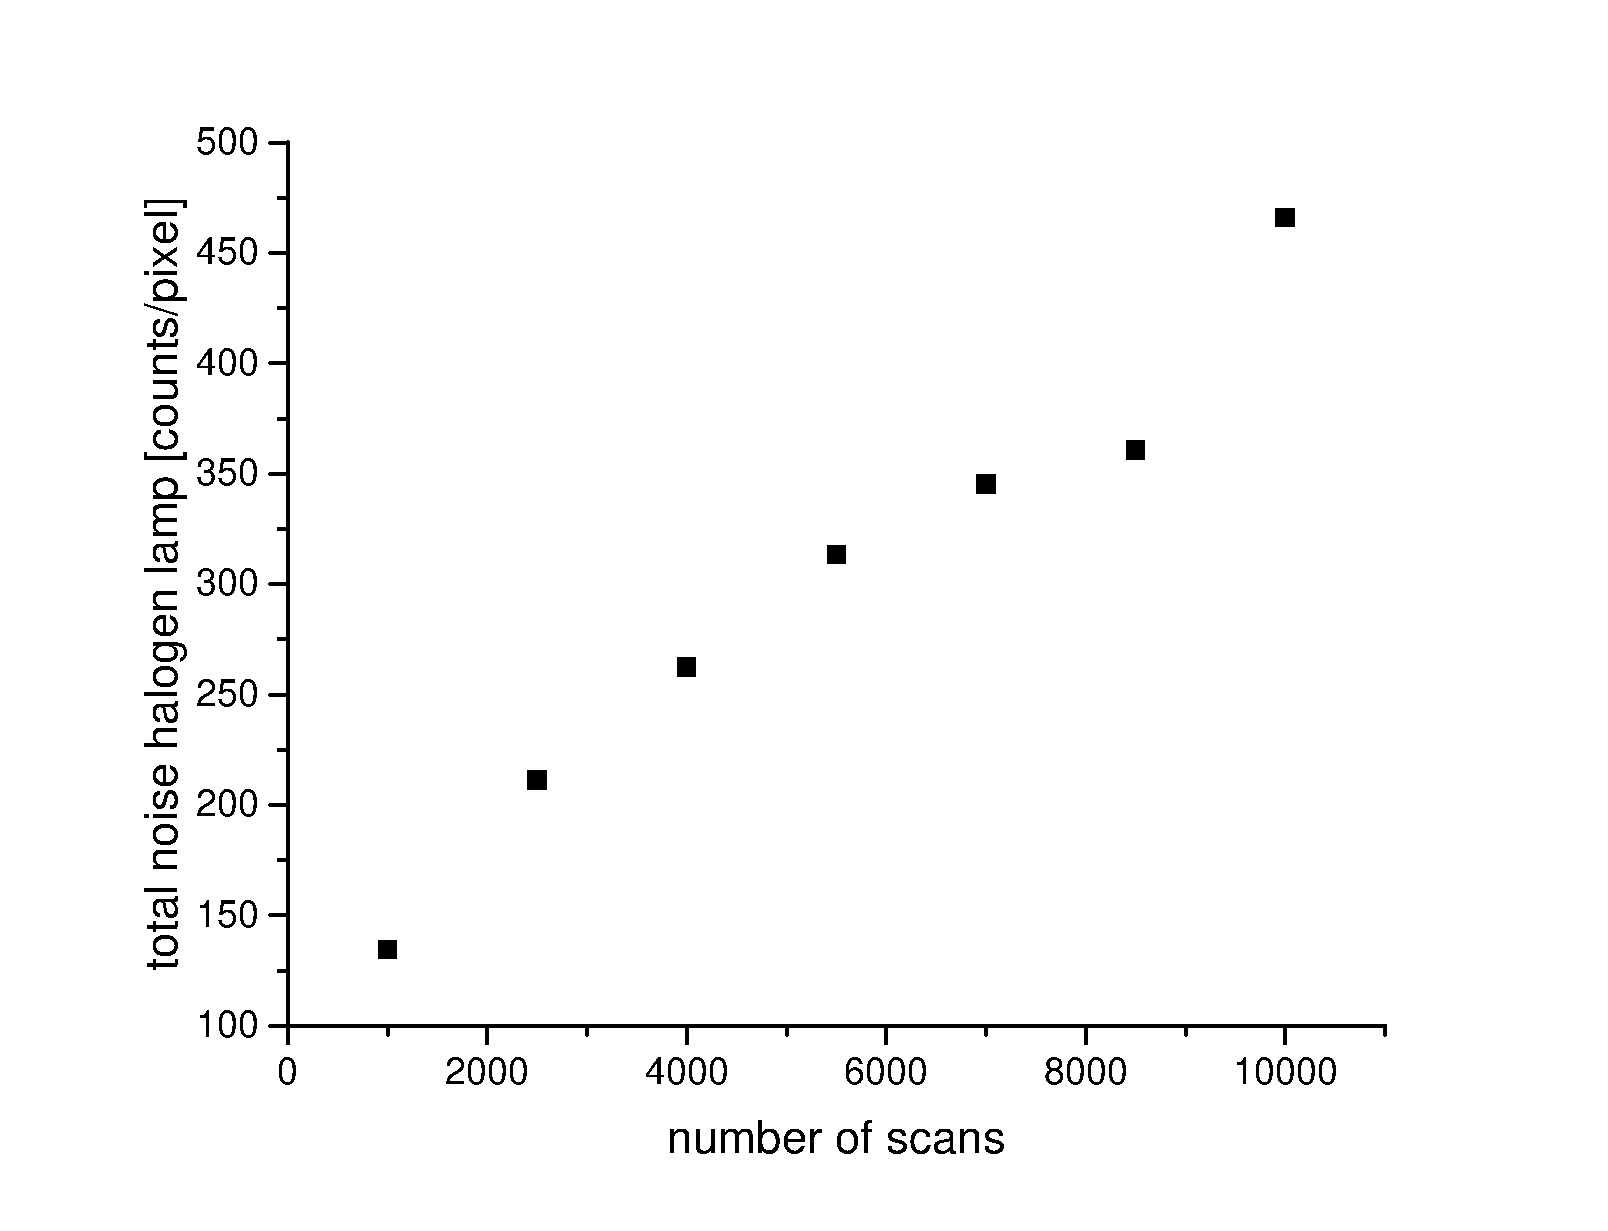
\includegraphics[width=\linewidth]{fig/total_noise_halogenlamp_plot.pdf}
	\captionof{figure}{Abhängigkeit des totalen Rauschens von der Anzahl der Scans}
	\label{fig:total_noise}
\end{center}  

Es zeigt sich in Abbildung \ref{fig:total_noise} die gleiche Charakteristik wie in Abbildung \ref{fig:instrumental_noise}. Lediglich die Stärke des Rauschen unterscheidet sich, was aber zu erwarten war, da im totalen Rauschen auch das Instrumentenrauschen integriert ist.
\\
Eine weitere Untersuchung der Halogenlampenspektren ermöglicht einen Einblick in die optische Dichte des relativen totalen Rauschens. Dazu wurden die zuvor aufgenommenen Spektren durcheinander geteilt und anschließend der Logarithmus des Ergebnisses betrachtet.

\begin{center}
    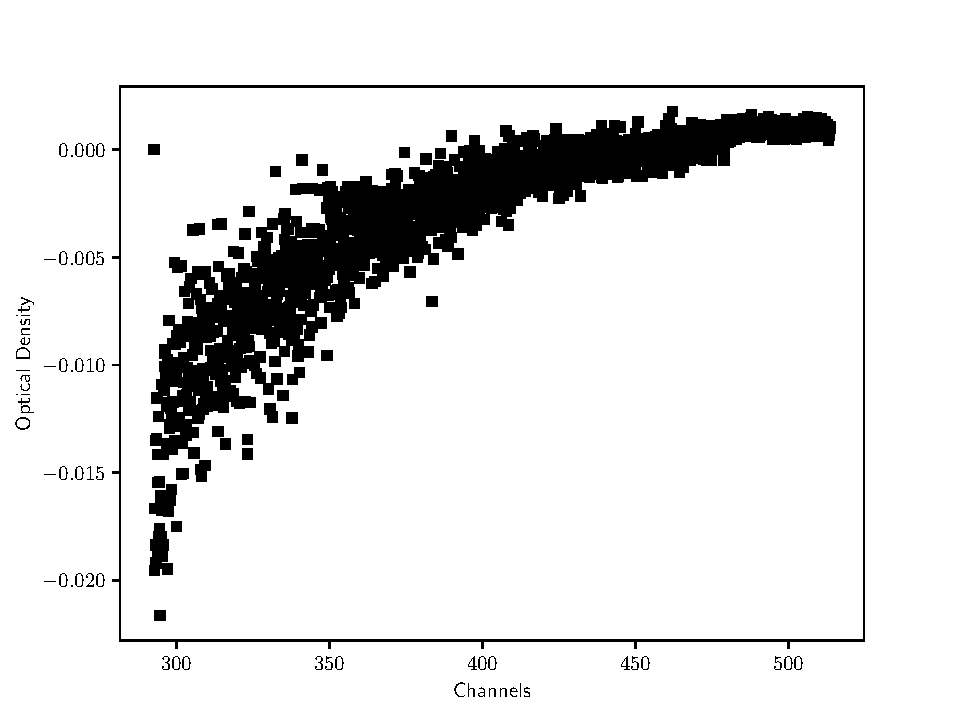
\includegraphics[width=\linewidth]{fig/hal_log.pdf}
    \captionof{figure}{Optische Dichte der Halogenlampe}	
    \label{fig:hal_log}
\end{center}

Man erwartet, dass der Mittelwert bei Null liegt, da zwischen der Aufnahme der Spektren so wenig wie möglich Zeit vergangen ist. Allerdings kann bei kleinerer Channelzahl höhere Schwankungen ausgemacht werden und insgesamt ist ein kurven artiger Verlauf zu erkennen.
Das größere Schwanken lässt sich darauf zurückführen, dass bei kleiner Channelzahl die \textit{Counts} geringer ausfallen als bei höherer Channelzahl.
Durch Schwankungen der Halogenlampenintensität ensteht in den Daten die beobachtete Krümmung, welche bei höherer Scanzahl größer wird. Die Schwankungen verlieren bei höheren \textit{Counts} an Bedeutung.

\subsubsection{Kalibrierung des Spektrometers}\label{sssec:calibrating_the_spectrometer}

Zur Kalibrierung des Spektrometers wird eine Quecksilberdampflampe verwendet, da diese gut zu identifizierende Spektrallinien aufweist.
Das aufgenommene Spektrum (siehe Abbildung \ref{fig:hg_spectrum}) wurde nach bekannten Spektrallinien untersucht und anhand von vier Maxima (entsprechend den Channelnummern: 335, 595, 946, 1239) das Spektrometer kalibriert. 


\begin{center}
    %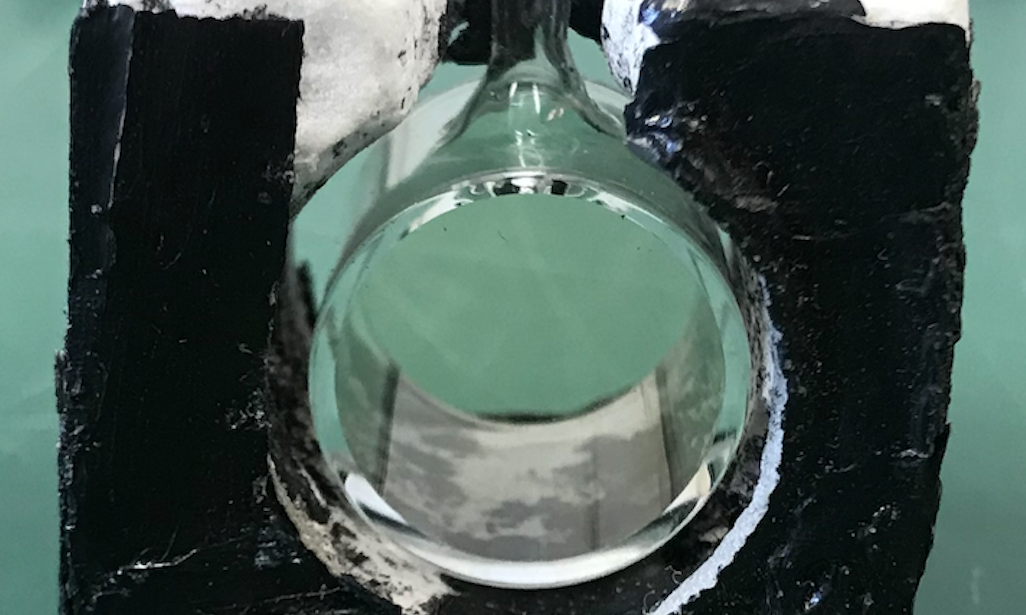
\includegraphics[width=0.7\linewidth]{fig/photo/glas.png}
    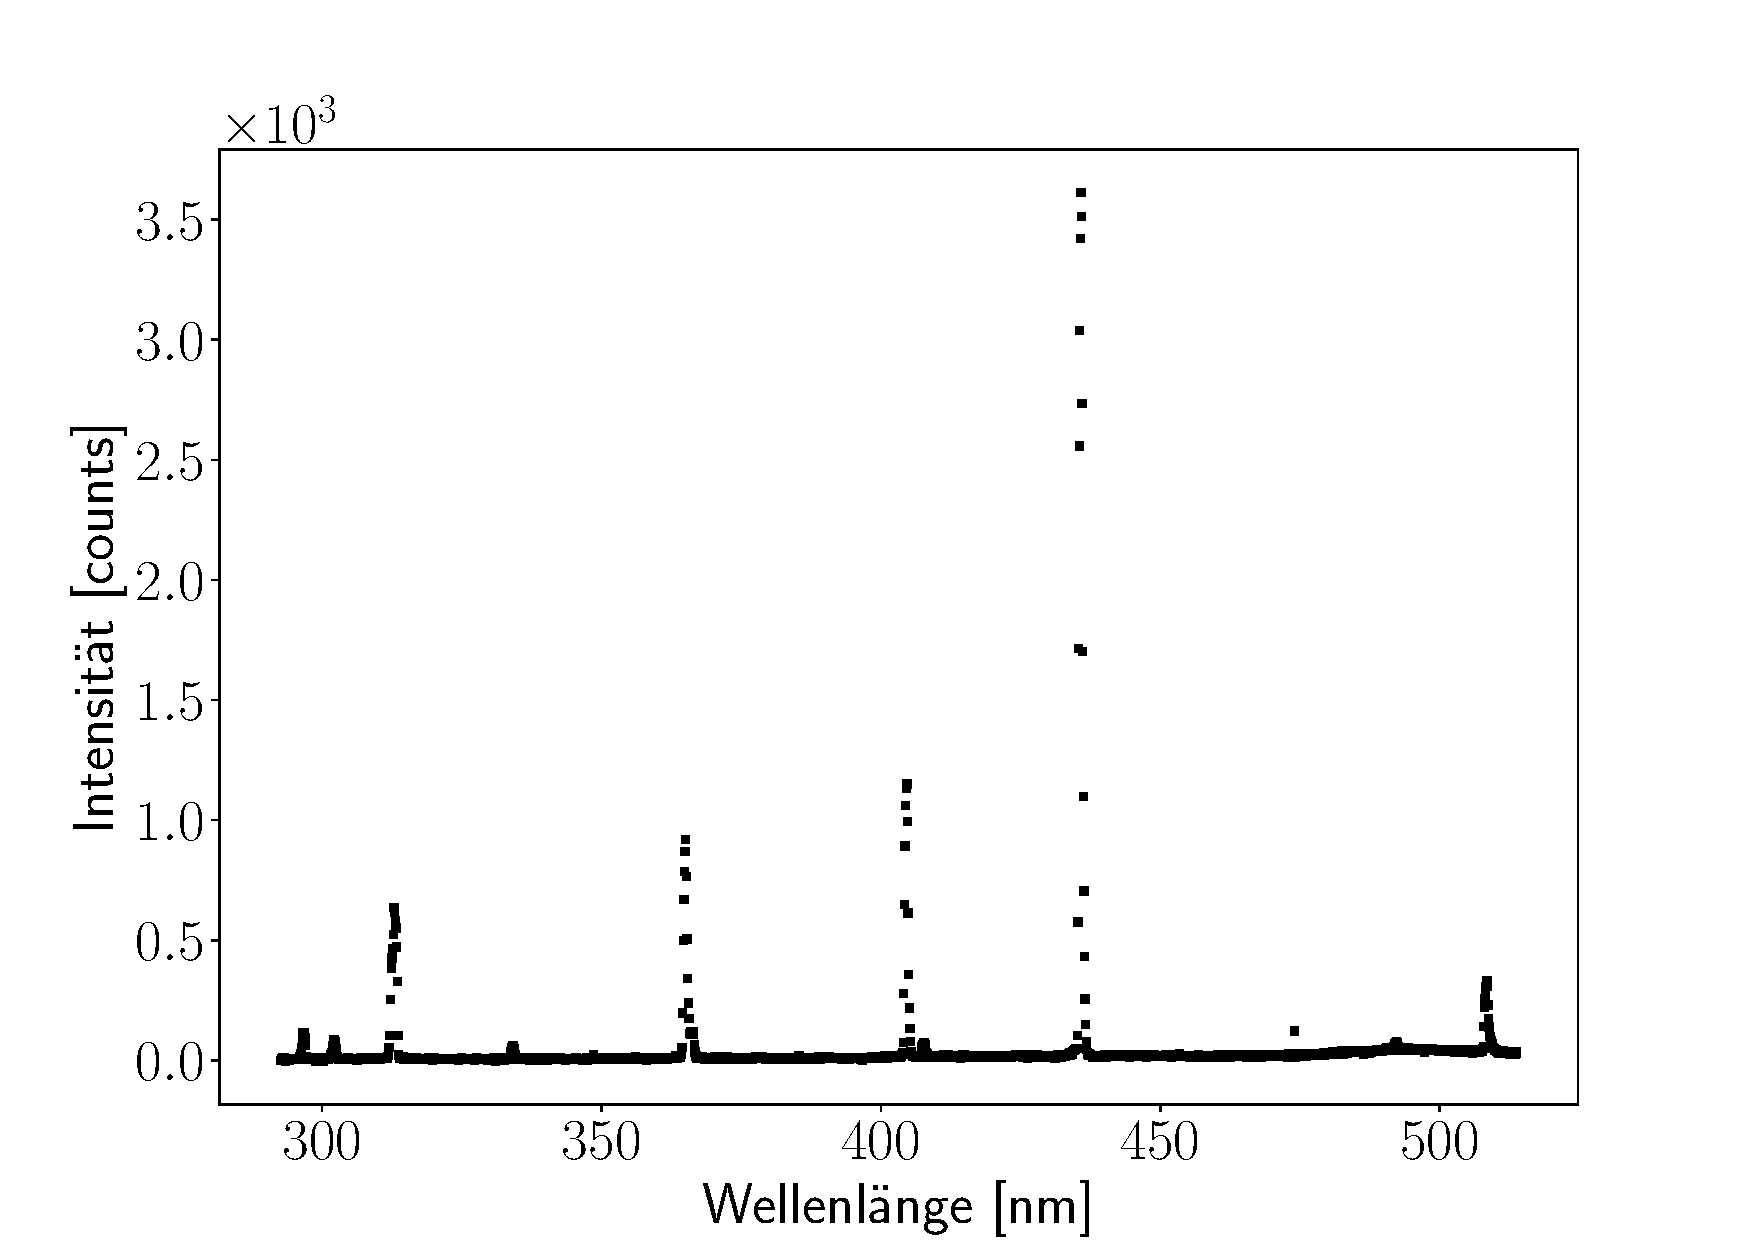
\includegraphics[width=\linewidth]{fig/hg_spectrum.pdf}
    \captionof{figure}{Spektrum der Quecksilberlampe}	
    \label{fig:hg_spectrum}
\end{center}



Es wäre ebenfalls eine Spektrallinie bei ca. $313$ \si{nm} gegeben. 
Diese wurde allerdings nicht zur Kalibrierung verwendet, da man aus der Literatur herauslesen kann, dass an dieser Stelle in Wirklichkeit drei verschiedene Linien zu finden sind \cite{doas08}.\\
Für die Kalibrierung wird ein Polynom zweiter Ordnung genutzt mit folgenden Parameter: 

\begin{align}
    \text{coeff}_0 &= 292.61 \pm 0.043611, \\
    \text{coeff}_1 &= 0.12726 \pm 0.00016266, \\
    \text{coeff}_2 &= 9.3859 \cdot 10^{-6} \pm 1.193 \cdot 10^{-7}. 
\end{align}
 
Über die \textit{full width at half max} (FWHM) lässt sich nun die optische Auflösung des Spektrometers bestimmen.

\begin{center}
	
\begin{tabular*}{\linewidth}{@{\extracolsep{\fill}} c c c}
	\toprule
	Maximum & Wellenlänge & FWHM [\si{nm}] \\
	\midrule
	1 & $\sim 313$ & $1.2 \pm 0.1$ \\
	2 & $\sim 365$ & $0.8 \pm 0.1$ \\
	3 & $\sim 404$ & $0.6 \pm 0.1$ \\
	4 & $\sim 436$ & $0.7 \pm 0.1$ \\
	\bottomrule
\end{tabular*}

	\captionof{table}{Optische Auflösung der verschiedenen Maxima} %\cite{atm_components}
	\label{fig:optical_resolution}
\end{center}

Bei der Analyse der FWHM stellt sich heraus, dass die optische Auflösung des Spektrometers bei höherer Channelzahl besser wird, deshalb wird versucht in den folgenden Messungen die Analyse, wenn möglich, im hohen Channelbereich durchzuführen.

\subsection{Labormessungen}\label{ssec:Labormessungen}

\subsubsection{Anpassung von Referenzspektren}\label{sssec:convolution_of_reference}

Mithilfe eines Literaturspektrums kann ein Vergleichsspektrum generiert werden. 
Die verwendeten Literaturspektren haben allerdings unterschiedliche Auflösungen und daher muss man diese entsprechend skalieren.
Dies kann mithilfe einer Faltung erledigt werden.
Die Faltung einer Funktion $f$ mit einer Funktion $g$ ist definiert als

\begin{align}
    (f \ast g) (x) := \int f(y) g(x-y) \dd y .
\end{align}

% Die Faltung sorgt zusätzlich dafür, dass das Spektrum geglättet wird.
Wellenlängen die außerhalb des Bereiches der Messgeräte liegen werden durch die Faltung abgeschnitten.\\
Es wurden Spektren von  \ch{CO2}, \ch{H2O}, \ch{O3} und \ch{O4} angepasst.
Das Referenzspektrum von \ch{H2O} wurde, im Gegensatz zu den anderen Spektren, vergrößert. 
Hierfür wurden Nullwerte an den Rändern angefügt.\\
Die Faltung hat zusätzlich noch den Effekt, die Spektren zu glätten.

\subsubsection{\ch{NO2} Spektrum einer gefüllten Glasküvette}\label{sssec:lab_no2_spectra}

Um die in den vorigen Abschnitten durchgeführten Vorbereitungen zu testen wird das Spektrum einer Halogenlampe untersucht, bei der eine Glasküvette, mit \ch{NO2} gefüllt, in den Lichtweg gestellt wird.
Die Glasküvette hatte eine Länge von ungefähr $2$\si{cm}.
Es wurden folgende Abstände eingestellt:
\begin{center}

\begin{tabular*}{\linewidth}{ @{\extracolsep{\fill}} c c}
	\toprule
    Objetkte & Abstand \si{[cm]} \\
	\midrule
    Kamera - Linse & 6.7\\
    Linse - Küvette & 4.3 \\
    Linse - Halogen & 12.6 \\
	\bottomrule
\end{tabular*}
    \captionof{table}{Eingestellte Abstände bei Messung mit Halogenlampe} %\cite{atm_components}
    \label{fig:distances}
\end{center}

\begin{center}
    %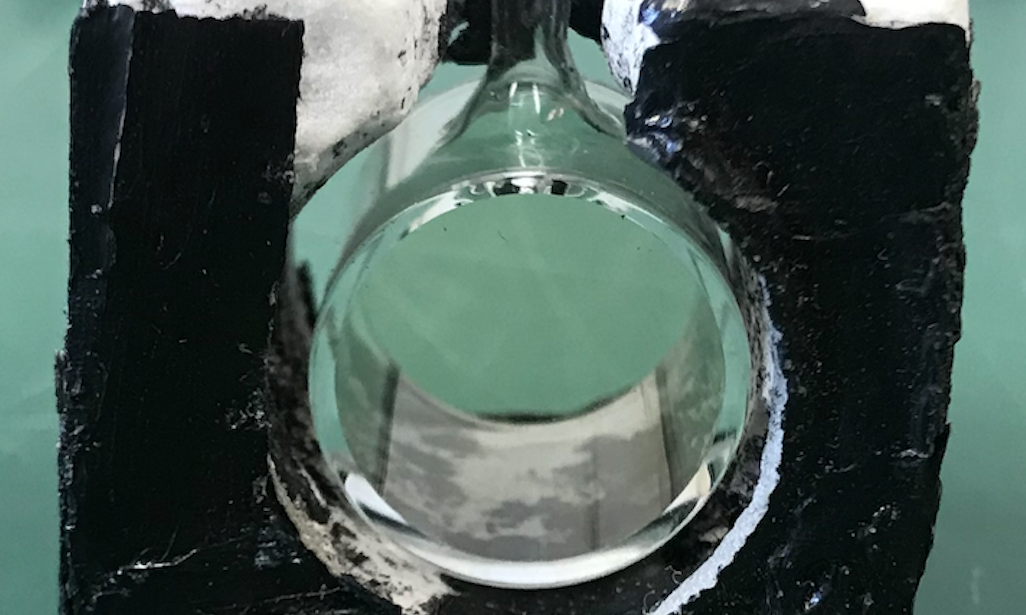
\includegraphics[width=0.7\linewidth]{fig/photo/glas.png}
    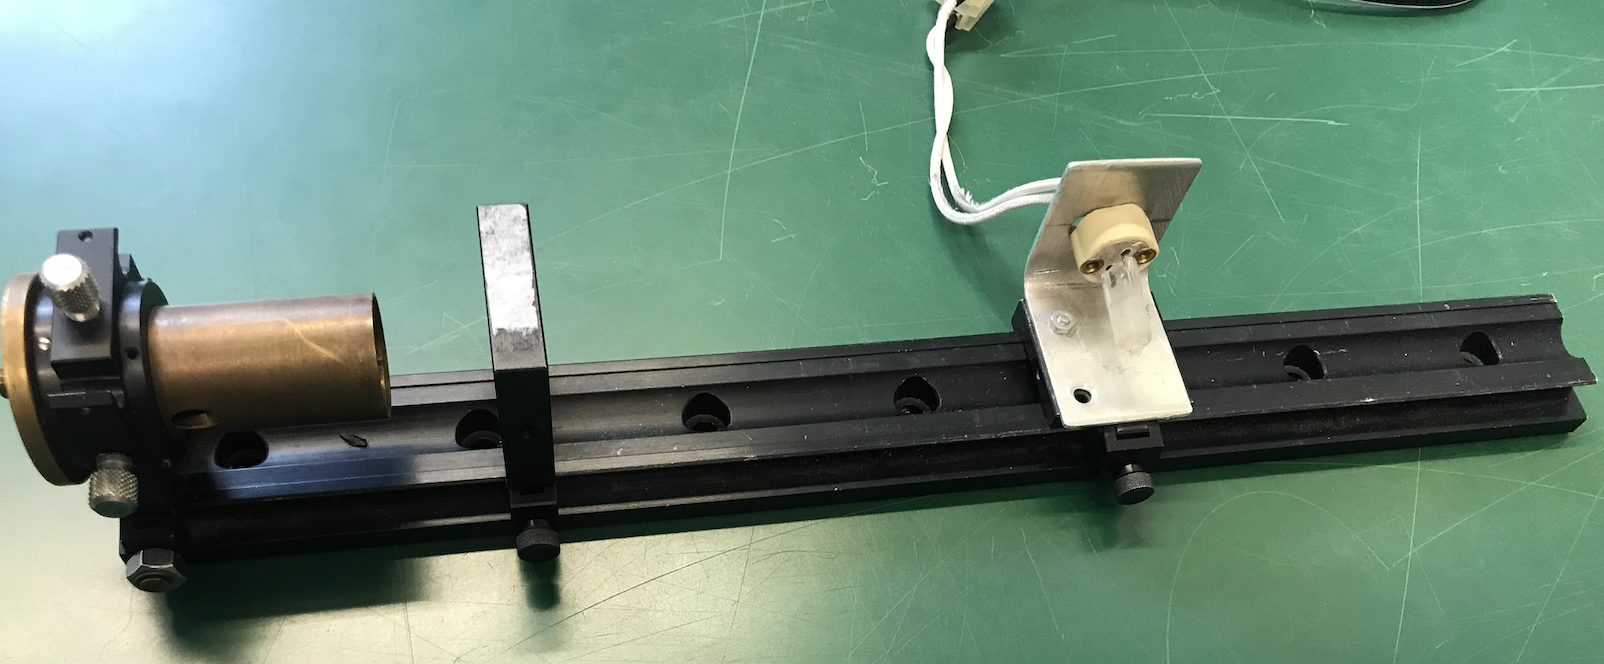
\includegraphics[width=\linewidth]{fig/photo/aufbau_1.png}
    \captionof{figure}{Versuchsaufbau}	
    \label{fig:aufbau_hal}
\end{center}


Mithilfe des Lambert-Beer Gesetztes lässt sich nun über die optische Dichte innerhalb der Gasküvette die Konzentration bestimmen (vgl. Gleichung \eqref{eq:lambert_beer_law} und \eqref{eq:optical_density})

\begin{align}
\tau = \ln(\frac{I_0(\lambda)}{I(\lambda)}) = \sigma_{\ch{NO2}}(\lambda) \cdot \rho_{\ch{NO2}} \cdot L.
\end{align}

Bei der Aufnahme der Spektren ist zu beachten, dass kein Teilbereich in Sättigung ist.
Sollte eine Anpassung der Anzahl der Scans oder der Sättigung nötig sein, ist dies ohne weiteres möglich. 
Dies liegt daran, dass Änderung der Parameter sich auf die Intensitäten als Faktor niederschlägt. 
Aus dem Lambert-Beer Gesetz folgt
\begin{align}
    \log \left( \frac{m}{n} \frac{I_\text{F} I_{0, i}}{I_i I_{0, \text{F}}} \right) = \log \left(\frac{m}{n} \text{e}^{(\sigma \rho \Delta L)}\right) ,
\end{align}
wobei $m$ und $n$ hier für die verschiedenen Scananzahlen und Sättigungen stehen. 
$I_\text{F}$ bezeichnet das Fraunhoferspektrum und $I_i$ ein beliebiges aufgenommenes Spektrum.
$I_{0, \text{F}}$ und $I_{0, i}$ sind gleich.
\\
Über einen \textit{least-square-fit} wird nun die SCD so variiert, dass das $\chi^2$ minimiert wird. 
In \ref{fig:different_fit_ranges} wurden die Fitparameter bei verschiedenen Fitbereichen betrachtet. 
Dabei wurde immer ein Polynom 5. Grades ohne Offset gefittet.
Den optimalen Fitbereich lässt sich über eine Überlagerung (siehe Abbildung \ref{fig:range_search}) des aufgenommenen Spektrums mit dem \ch{NO2} Referenzspektrum finden.

\begin{center}
	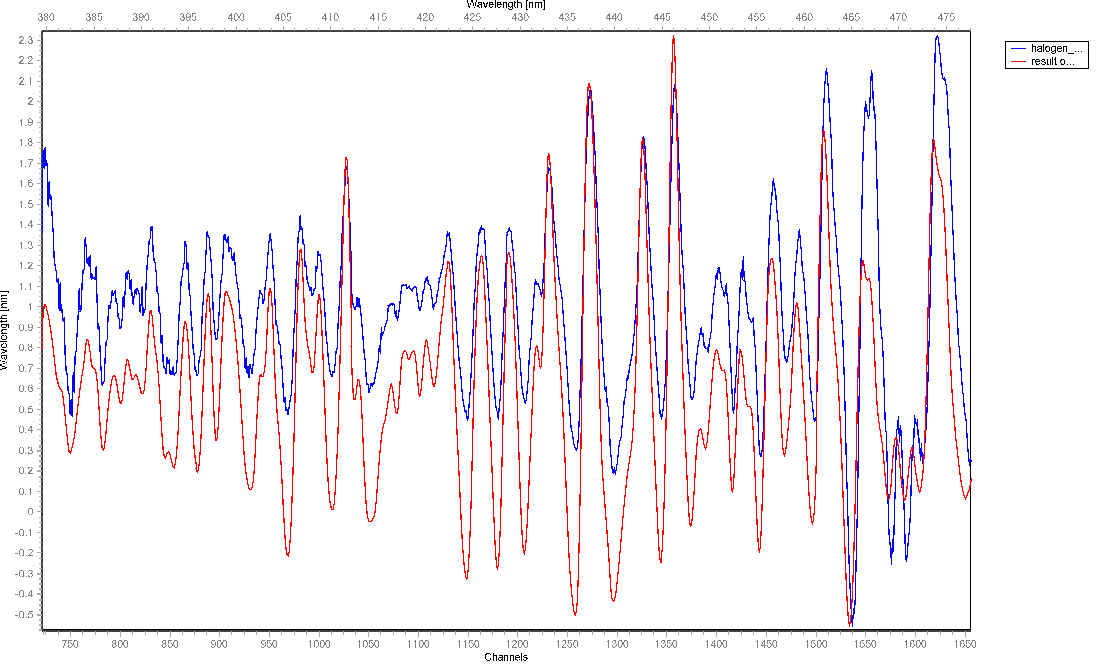
\includegraphics[width=\linewidth]{fig/range_search_test.png}
	\captionof{figure}{Überlagerung des aufgenommenen und des Referenz- Spektrums}
	\label{fig:range_search}
\end{center}

Die Überlagerung zeigt im Channelbereich $1000-1700$ die gleichen Strukturen. Der Fit wird in diesem Bereich durchgeführt.
Für die genau Bestimmung der \ch{NO2} Konzentration wurde ein Channelbereich von $1026-1663$ ausgewählt, was einem Wellenlängenbereich von $413.46 - 477.25$ \si{nm} entspricht.
Dabei wurde darauf geachtet, dass die Intensität bei einer Wellenlänge von $470$\si{nm} ca. $80$\% betrug.
Damit konnten beim Fit die Parameter

\begin{align}
	\chi^2 &= 4.367 \cdot 10^{-3},\\
    \text{fit coeff} &= -4.96 \cdot 10^{17} \pm 1.95 \cdot 10^{15},\\
    \text{shift} &= 0.0955 \pm 0.00538,\\
    \text{squeeze} &= 0.993 \pm 0.000159, 
\end{align}

erreicht werden.
Mit der nun bestimmten \textit{slant column density} kann nun die \ch{NO2} Konzentration in der Küvette berechnet werden.
Die Länge wurde von Hand auf $2.0 \pm 0.1$\si{cm} bestimmt, sodass sich mit der Gaußschen Fehlerfortpflanzung eine Konzentration von

\begin{align}
    \rho_{\ch{NO2}} = (2.48 \pm 0.12) \cdot 10^{20} \Bigl[ \frac{\text{Moleküle}}{\ell}\Bigr]
\end{align}

ergibt.	
Ebenfalls lässt sich nun das Mischverhältnis auf

\begin{align}
    R &= \frac{\rho_{\ch{NO2}}}{\rho_{\text{std}}-\rho_{\ch{NO2}}}\\ 
    &= (9.311 \pm 0.004) \cdot 10^{-3}\\
    &= 9.311 \pm 0.004 \si{ppt}
\end{align}

beziffern. Dazu wurde die $\rho_{\text{std}}$ aus den Normalbedingungen gewonnen.

\begin{align}
    \rho_{\text{std}} = \frac{N_A}{V_M}.
\end{align}
 	
Mit $N_A = 6.022 \cdot 10^{23} \frac{1}{\si{mol}}$ und $V_M = 22.4 \frac{\ell}{\si{\mol}}$.

\subsection{Atmosphärische Messungen}\label{ssec:atmospheric_measurements}

Nachdem man sich nun mit dem Messverfahren und der Analyse der Daten vertraut gemacht hat, werden nun atmosphärische Spurengase untersucht. In diesem Praktikumsversuch beschränkt man sich auf \ch{O3} und \ch{NO2}.
Für die Analyse wurde ein Tag ausgesucht bei dem gutes Wetter herrschte, sodass Wolken nicht die Messung beeinträchtigen können; über einen langen Zeitraum aufgenommen wurde; sowie nicht zu weit in der Vergangenheit lag, da man einer möglichen Abweichung von Dunkelstrom und Offset minimieren wollte.
Die Wahl fiel auf den 23.04.2019, wo über einen Zeitraum von $9:13 - 23:56$ UTC aufgenommen wurde.

\subsubsection{Optimierung des Fitalgorithmus}\label{sssec:configure_fit}

Die für die \verb*+DOASIS+ nötige Referenzmessung, die Fraunhoferreferenz, wurde die Tagesmessung mit dem niedrigsten
\textit{solar zenith angle} (SZA) ausgewählt. 
Da der statistische Lichtweg hier am kürzesten ist und somit am wenigsten von möglichen Spurengasen absorbiert wurde.
Um nun die Parameter des Fits optimal anpassen zu können, wird ein Spektrum bei $80$ SZA ausgewählt um die größtmögliche Differenz zwischen den beiden Spektren zu erzeugen. 
Dies gewährleistet, dass die zu untersuchenden Strukturen am prägnantesten hervortreten. \\
Um dem Ringeffekt (vgl.\ref{ssec:Kurzband}) zu berücksichtigen, wird ein \textit{Ringspektrum} $R(\lambda)$ aus dem Fraunhoferspektrum berechnet.
Aus einer Berechnung der optischen Dichte und dem Vergleich mit den Referenzen der Spurengase (vgl. Abschnitt \ref{sssec:lab_no2_spectra}) werden wieder die jeweiligen Fitbereiche ermittelt. 
Die Fitbereiche sind in Tabelle \ref{fig:fit_of_atmospheric_data} aufgelistet.\\
Der Fitalgorithmus greift nun auf das Fraunhoferreferenzspektrum als erste Fit Referenz, dem Ringspektrum und den Referenzwirkungsquerschnitten der Spurengase zurück. 
Der Referenzwirkungsquerschnitt von \ch{H2O} kann bei \ch{O3} nicht verwendet werden, da es in diesen Bereichen Singularitäten aufweist.

\subsubsection{Untersuchung der Tagesmessung}\label{sssec:tagesmessung}

Nachdem die Fitbereiche optimiert wurden, werden die Daten des ganzen Tages untersucht. 
Hierbei standen $436$ Aufnahmen zur Verfügung.


\begin{center}
	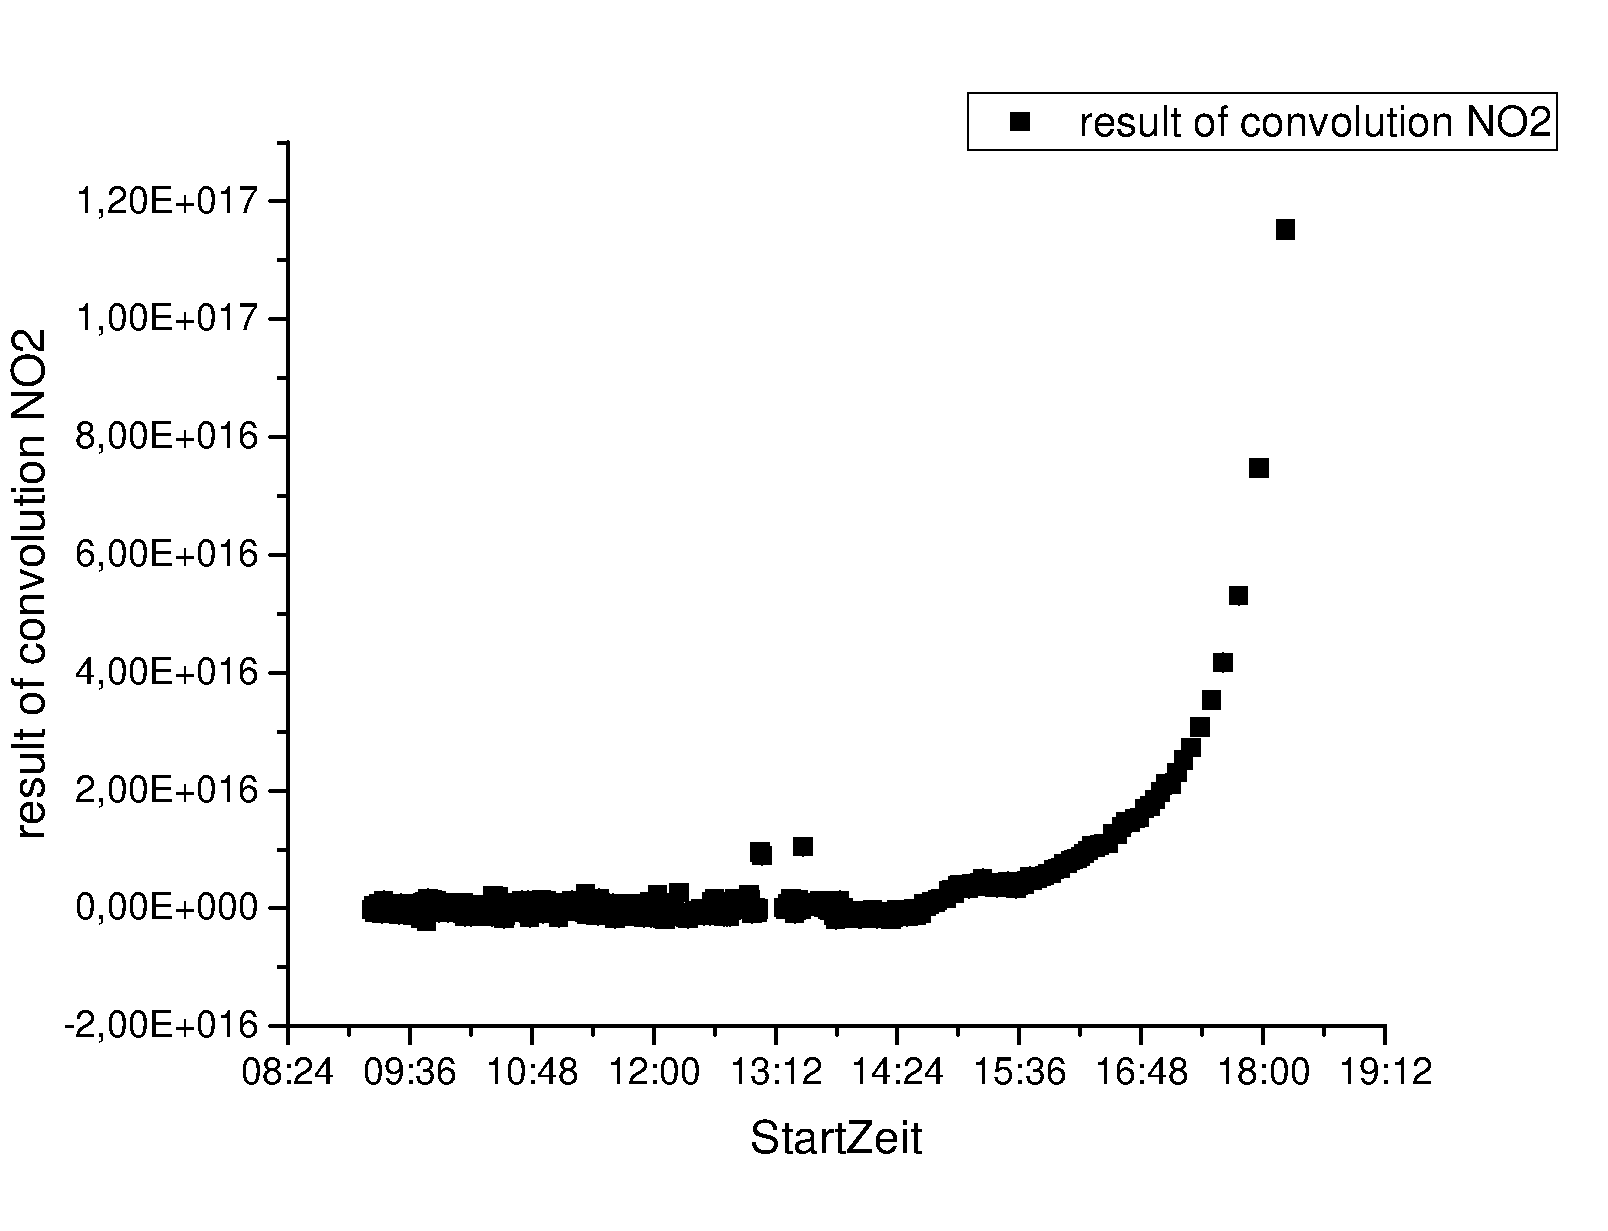
\includegraphics[width=\linewidth]{fig/SCD_Time_Plot_NO2.pdf}
    \captionof{figure}{$\Delta \text{SCD}$ von \ch{NO2} über den Tag des 24.04.2019}
	\label{fig:delta_SCD_time_NO2}
\end{center}
       
\begin{center}
	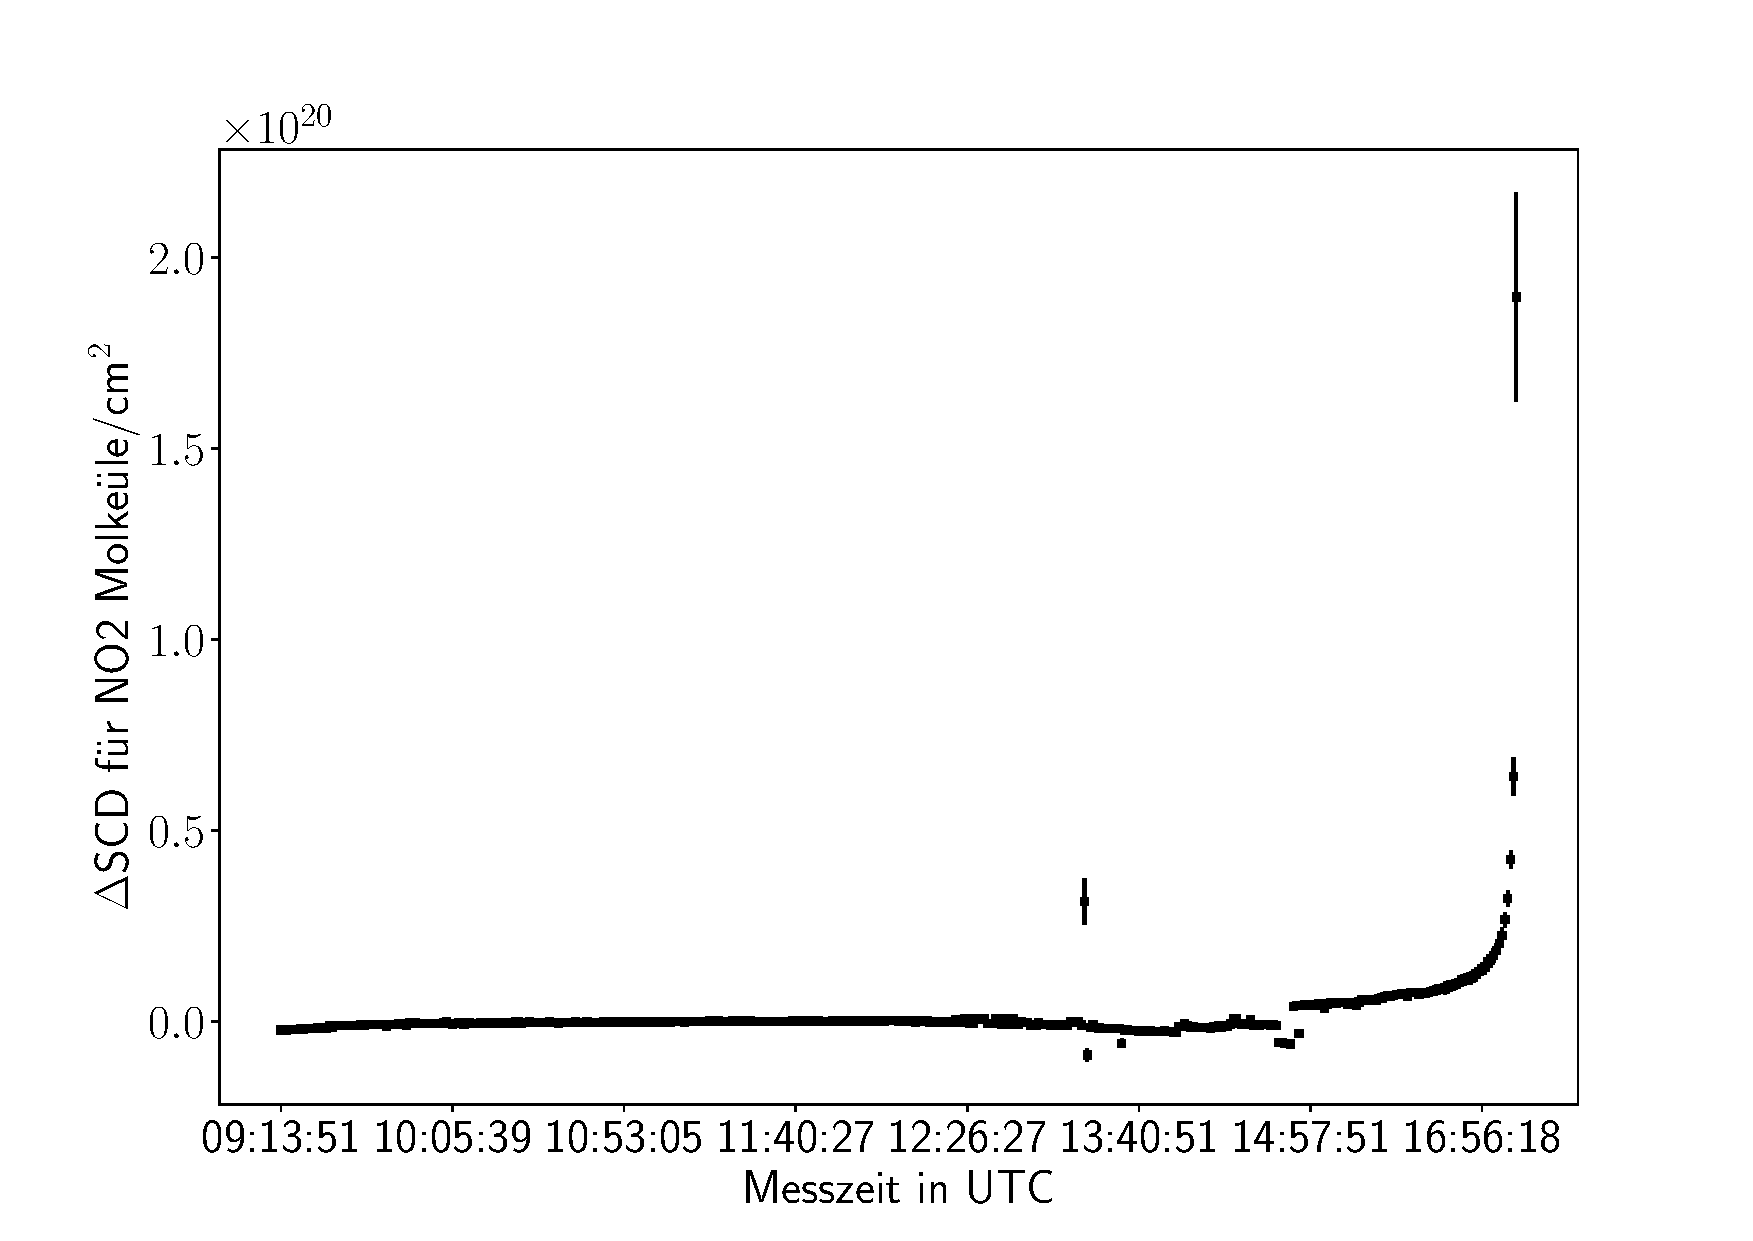
\includegraphics[width=\linewidth]{fig/SCD_Time_Plot_O3.pdf}
    \captionof{figure}{$\Delta \text{SCD}$ von \ch{O3} über den Tag des 24.04.2019}
	\label{fig:delta_SCD_time_O3}
\end{center}       

In Abbildung \ref{fig:delta_SCD_time_NO2} ist zu erkennen, dass $\Delta$SCD von \ch{NO2} zunächst niedrig ist, zum Abend hin jedoch stark zunimmt.\\
Grund dafür sind chemische Prozesse die Unterschiedlich stark bei verschiedener Sonneneinstrahlungen stattfinden.
Am Morgen (was hier nicht abgebildet ist) nimmt die Sonneneinstrahlung zu wodurch die Reaktion
\begin{align}
    \ch{NO2} + h \nu \to \ch{NO} + \ch{O} (^3\text{P}). \label{eq:creation_no}
\end{align}
vermehrt stattfindet.
Dadurch sinkt die Mischrate von \ch{NO2} zunächst.
Gleichzeitig kommt es zur Dissoziation 
\begin{align}
    \ch{N2O5} + h\nu \to \ch{NO2} + \ch{NO3},
\end{align}
wobei \ch{NO3} wieder weiter reagieren kann
\begin{align}
    \ch{NO3} + h\nu \to \ch{NO} + \ch{O2}, \\
    \ch{NO3} + h\nu \to \ch{NO2} + \ch{O}.
\end{align}
Diese Reaktionen treten vermehrt über den Tag auf, wodurch $\Delta$SCD wieder steigt. 
Bei den Messungen hier wurde erst am späten Vormittag begonnen, weswegen man nicht sehen kann, dass $\Delta$SCD morgens ebenfalls sehr hoch ist.
Ab 16:00 Uhr kann man einen starken Anstieg feststellen, welcher auf den Feierabend zurückzuführen ist.\\
Bei $\Delta$SCD von \ch{O3} in Abbildung \ref{fig:delta_SCD_time_O3} ist ein ähnliches verhalten zu beobachten.
In der Atmosphäre findet folgende Gleichgewichtsreaktion statt:
\begin{align}
    \ch{O3} + \ch{NO} \rightleftharpoons \ch{NO2} + \ch{O2}
\end{align}
Aus der Reaktion (\ref{eq:creation_no}) geht hervor, dass sich über den Tag die \ch{O3} Konzentration verringert, da mehr \ch{NO} entsteht.
Der Grund hierfür ist, dass die Reaktion (\ref{eq:creation_no}) über den Tag verstärkt vorkommt.
Es ist kein Einfluss durch den Feierabendverkehr wie in Abbildung \ref{fig:delta_SCD_time_NO2} zu erkennen, da \ch{O3} viel stärker in der Stratosphäre als in der Troposphäre vorkommt, sodass kleine \ch{O3} Änderungen nur im Fehlerbereich liegen.
\\
Eine Untersuchung der SCD gegen den \textit{Air Mass Factor}(AMF), lässt Rückschlüsse über eine Konzentrationsänderung über den Tag zu.

\begin{center}
	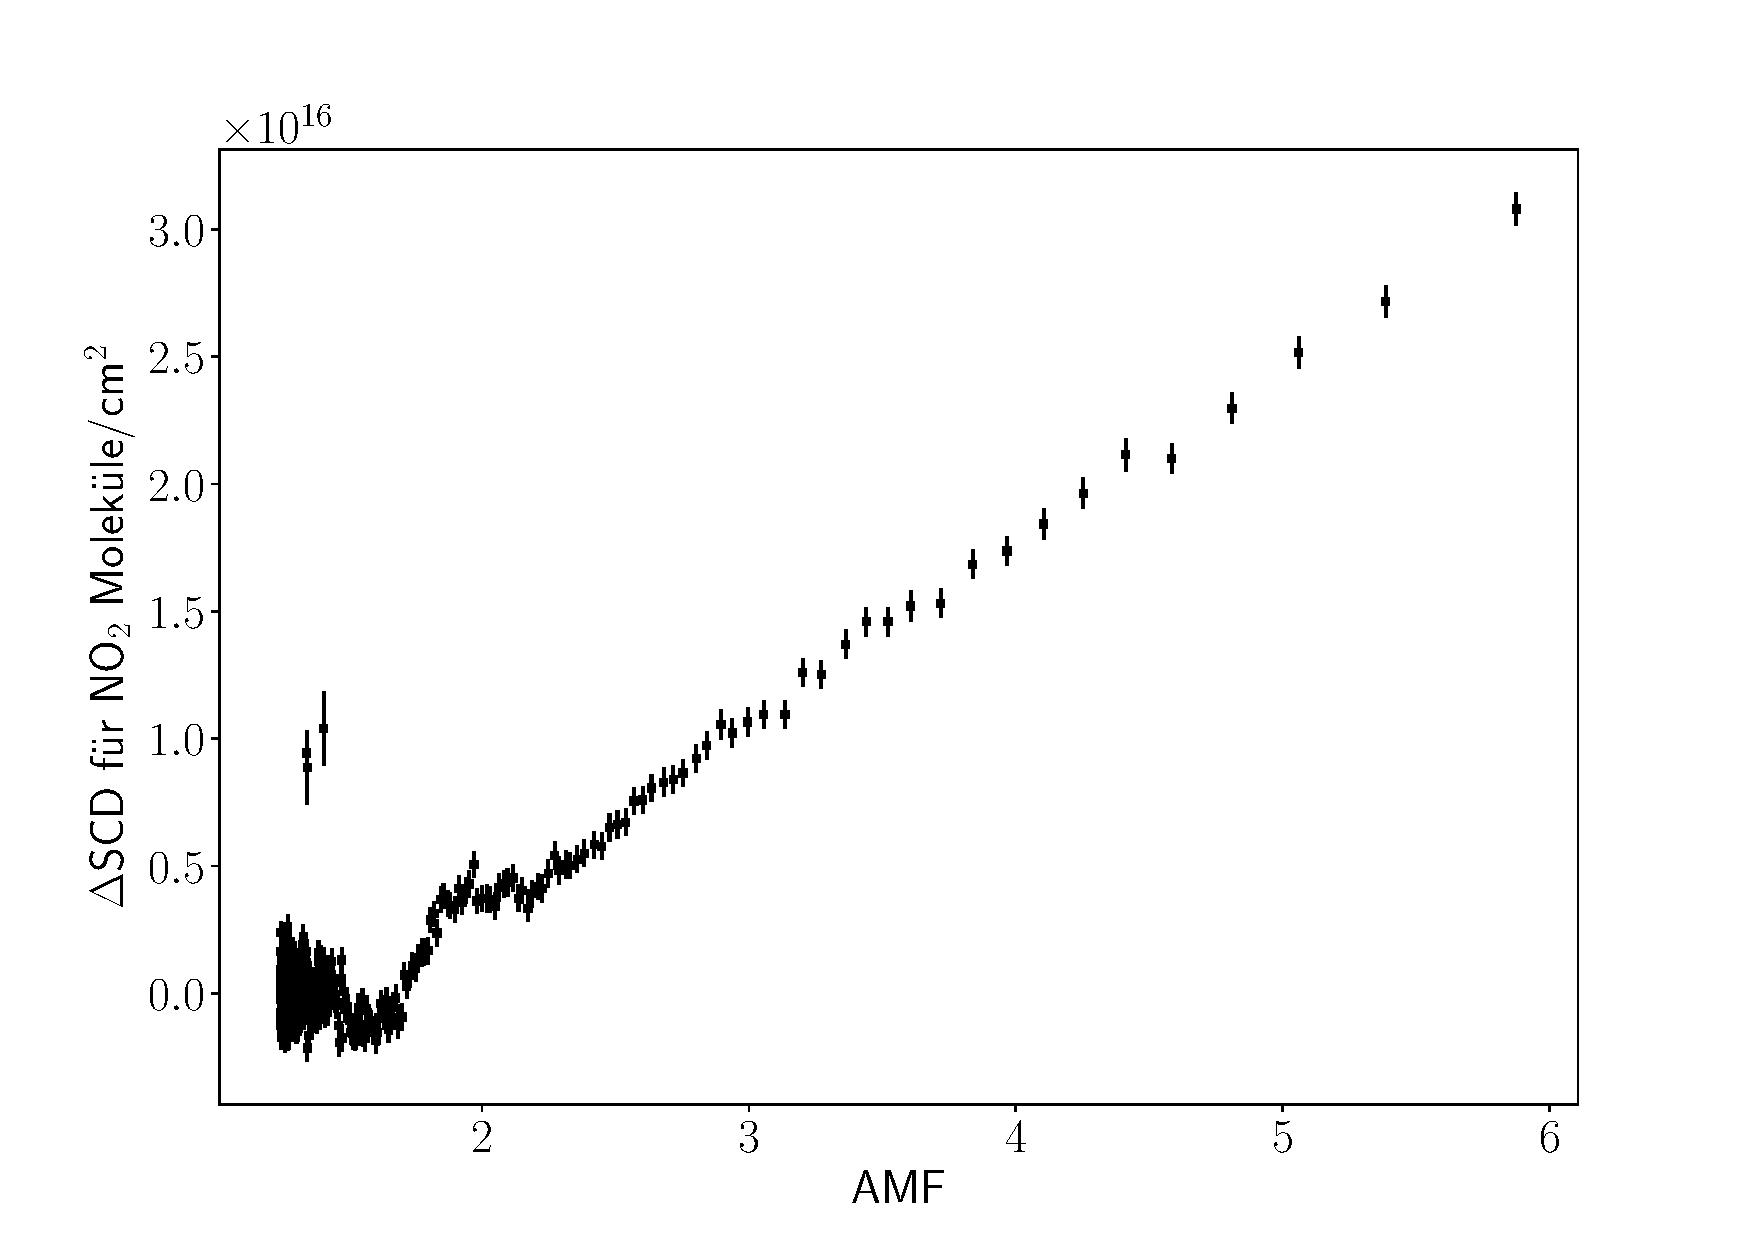
\includegraphics[width=\linewidth]{fig/Langley_Plot_NO2_cut.pdf}
	\captionof{figure}{Langley-Plot von \ch{NO2}}
	\label{fig:langley_NO2}
\end{center}

\begin{center}
	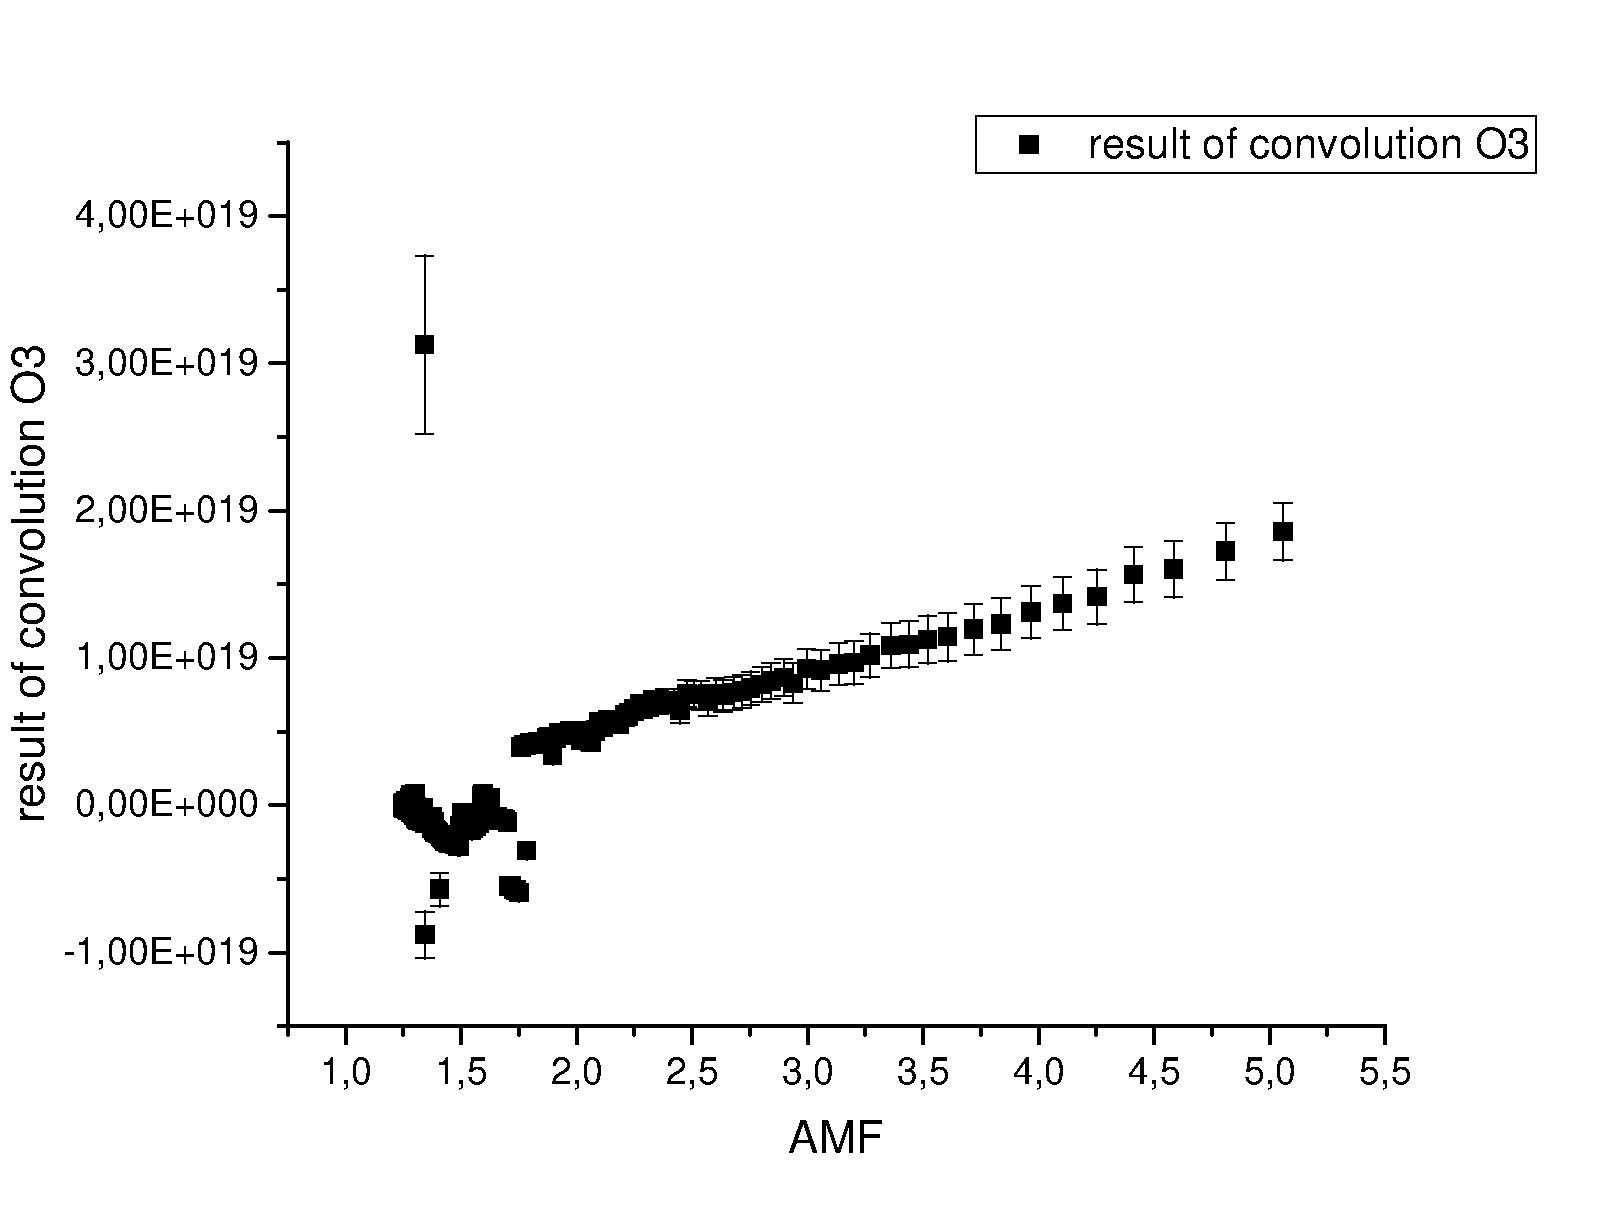
\includegraphics[width=\linewidth]{fig/Langley_Plot_O3_cut.pdf}
	\captionof{figure}{Langley-Plot von \ch{O3}}
	\label{fig:langley_O3}
\end{center}

Ein linearer Zusammenhang entspricht einer konstanten Konzentration über den Tag. 
Unsere Messdaten zeigen bei \ch{O3} als auch bei \ch{NO2} eine konstante Konzentration über den Tag.
Allerdings muss beachtet werden, dass Messungen vom Morgen nicht vorhanden sind.
Die Konzentration von \ch{NO2} ist, wie in Abschnitt \ref{sssec:tagesmessung} besprochen, am Morgen geringer als am Abend.
Wenn nun die Messungen vom Morgen im Langley-Plot vorhanden wären, könnte keine Gerade mehr eindeutig festgemacht werden, bei \ch{O3} lägen die Morgengerade und die Mittagsgerade übereinander.

\begin{center}
	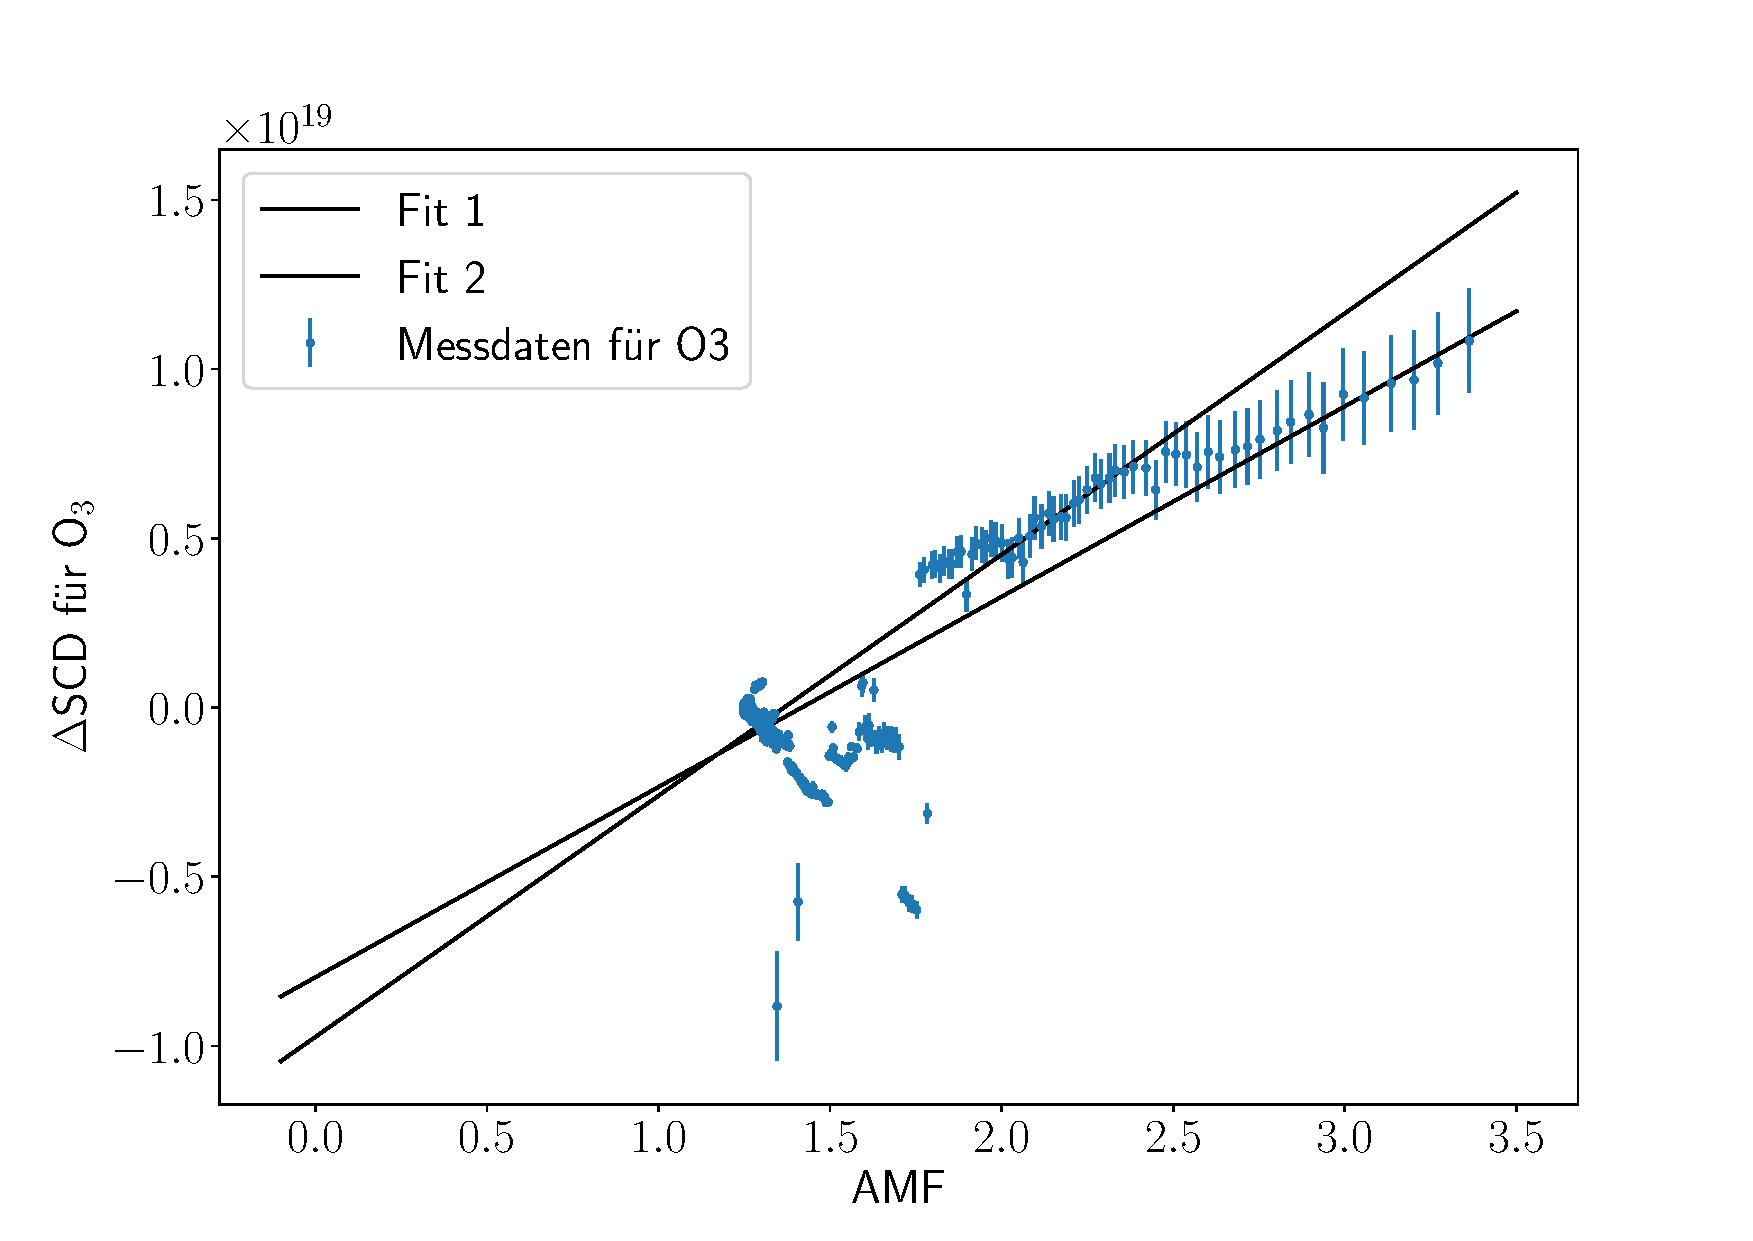
\includegraphics[width=\linewidth]{fig/scd_fit_o3.pdf}
    \captionof{figure}{$\Delta$SCD von \ch{O3} mit Fits.}
	\label{fig:scd_fit_o3}
\end{center}

Über einen Geradenfit im Langley Plot von \ch{O3} kann nun die $\text{SCD}_\text{ref}$, welche der y-Achsenabschnitt ist, abgelesen werden. Um einen Fehler aufgrund unserer schwankenden Messergebnisse zu erhalten wurde eine zweite zu rechtfertigende Gerade angegeben. Die Differenz der beiden y-Achsenabschnitte erlaubt es einen Fehler der $\text{SCD}_\text{ref}$ abzuschätzen.
 
\begin{align}
	\text{SCD}_\text{ref}= (0.97 \cdot 10^{19}\pm 0.17 \cdot 10^{19}) \si{\frac{Moleküle}{cm^2}}.
\end{align}	

Der horizontale Verlauf der \textit{vertical column density} (VCD) bestätigt die Aussage, dass die \ch{O3} Konzentration konstant über den Tag ist.

\begin{center}
	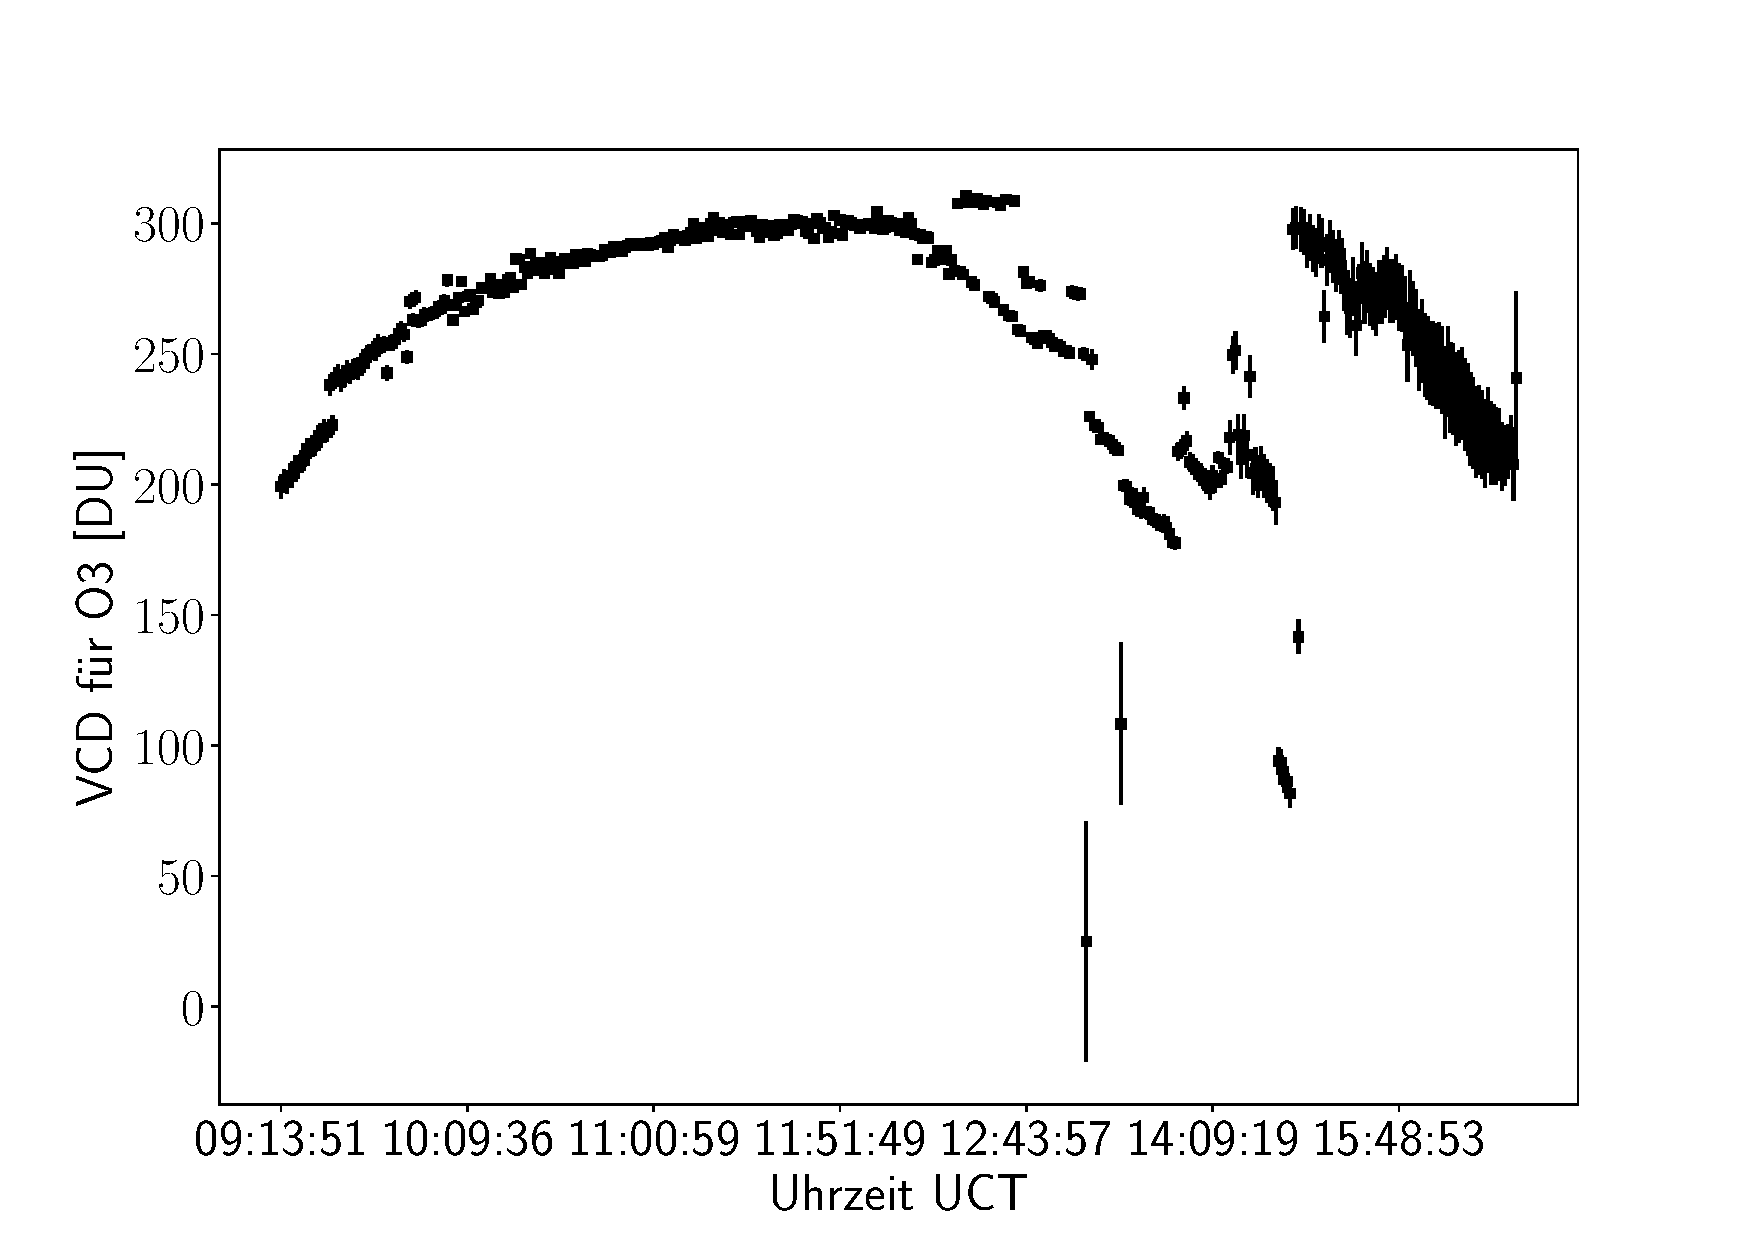
\includegraphics[width=\linewidth]{fig/VCD_O3_over_day.pdf}
    \captionof{figure}{VCD von \ch{O3} über einen Tag lang gemessen }
	\label{fig:VCD_O3_over_day}
\end{center} 

Die VCD berechnet sich dabei leicht über geometrische Zusammenhänge: 

\begin{align}
    \text{VCD} = ( \Delta \text{SCD} + \text{SCD}_\text{ref}) \cdot \cos(\theta)
\end{align}

\begin{center}
	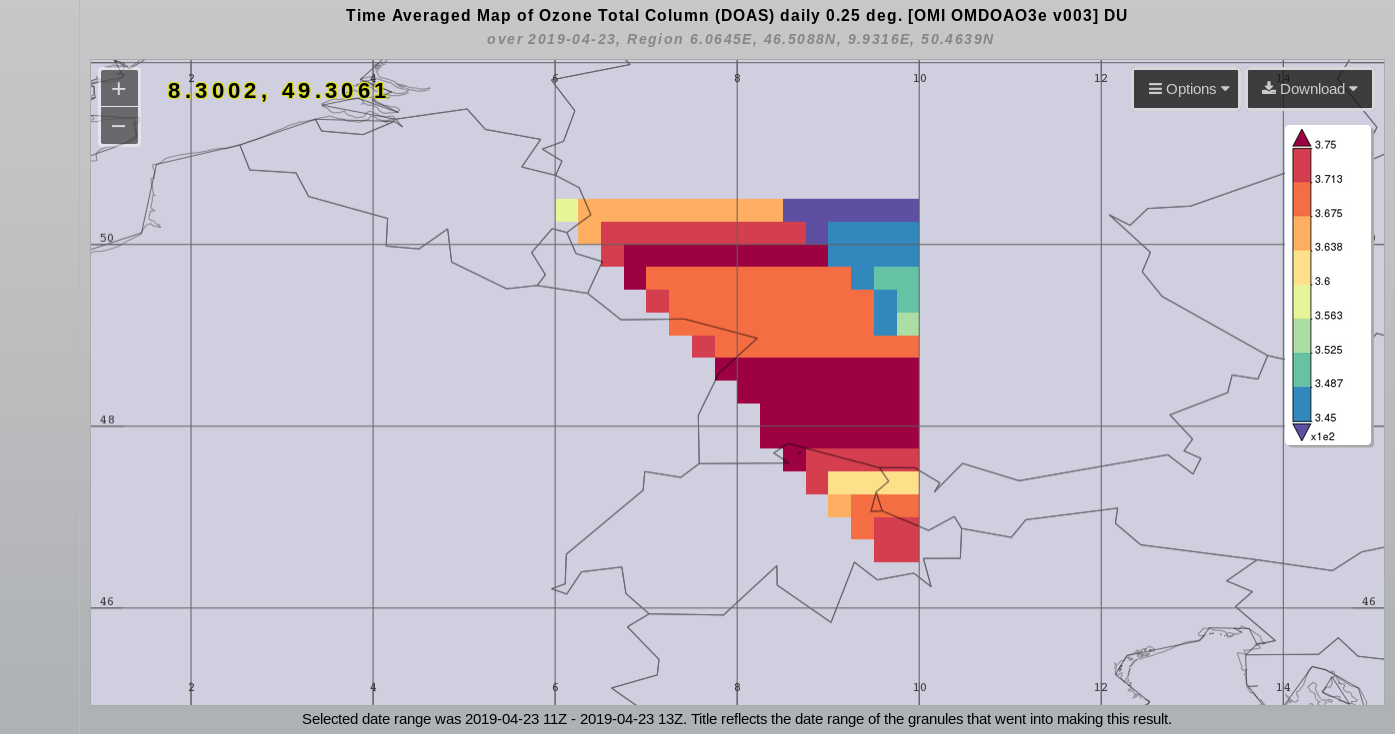
\includegraphics[width=\linewidth]{fig/DOAS_VCD_Ozone_ohne_Maus}
    \captionof{figure}{DOAS VCD Messung mit Satelit aufgenommen\footnotemark}
    \footnotetext{\url{https://disc.gsfc.nasa.gov/datasets/OMDOAO3G_V003/summary}}
	\label{fig:DOAS_satelit}
\end{center} 

\begin{center}
	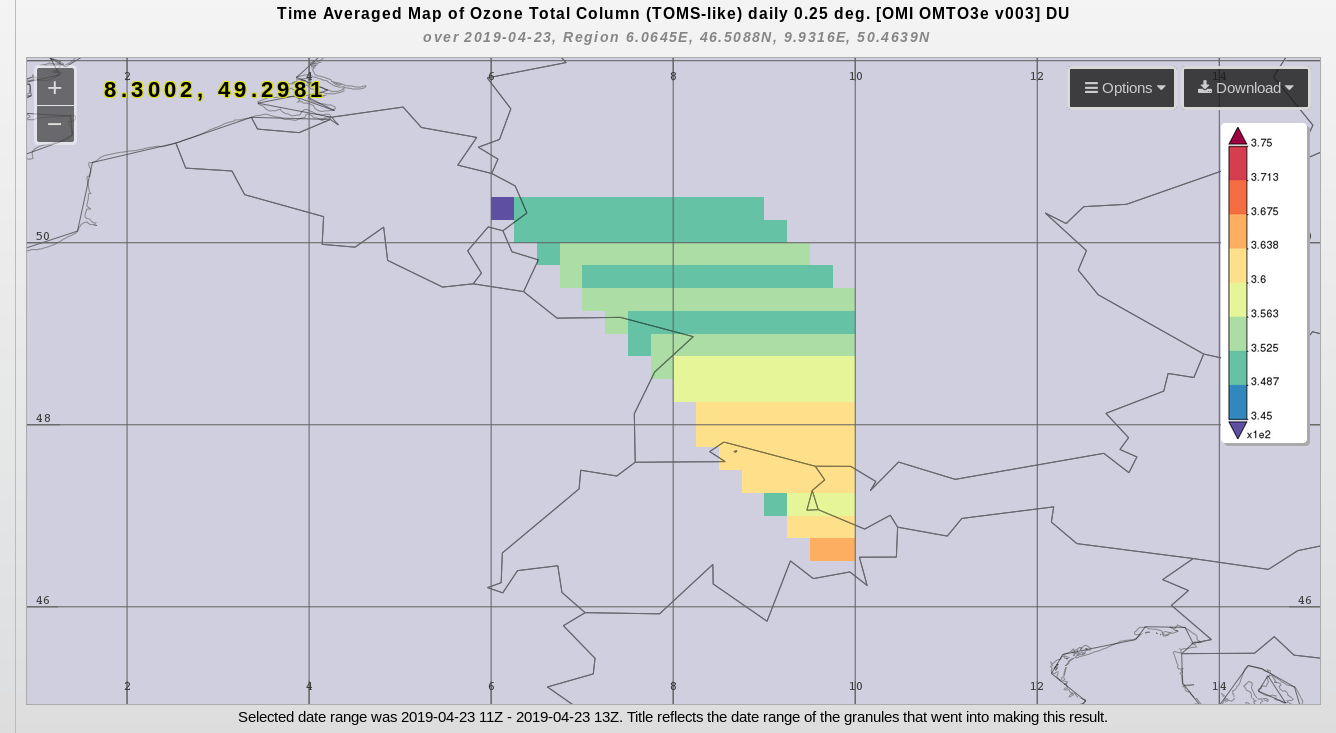
\includegraphics[width=\linewidth]{fig/TOMS_VCD_Ozone_ohne_Maus.png}
    \captionof{figure}{TOMS VCD Messung mit Satelit aufgenommen\footnotemark}
    \footnotetext{\url{https://disc.gsfc.nasa.gov/datasets/TOMSEPL3_V008/summary}}
	\label{fig:TOMS_satelit}
\end{center} 
Die beiden Satellitenbilder in Abbildung \ref{fig:DOAS_satelit} und \ref{fig:TOMS_satelit} zeigen die VCD Werte von Ozon über Baden-Württemberg am 23.04.2019.
DOAS zeigt bei den Koordinaten von Heidelberg einen Wert im Bereich von $363.8 - 367.5 \si{DU}$ an und TOMS einen Wert zwischen $352.5 \si{DU}$ und $358.3 \si{DU}$ an.
Die mit dem Satelliten aufgenommenen Werte sind also beide höher als die hier berechneten Werte.
Allerdings ist auch zu sehen, dass die Werte die beiden Messmethoden untereinander ebenfalls nicht übereinstimmen.
Abweichungen zu unseren Messwerten können dadurch entstehen, dass wir nur die Ozonkonzentration der Stratosphäre berechnet haben und die Troposphäre vernachlässigt wird, jedoch bei den Satellitenaufnahmen die gesamte Konzentration bestimmt wird.


\subsection{Multi Axis DOAS}\label{ssec:multi_axis_DOAS}

Einen Einblick in die vertikale Verteilung der Spurengase liefert die Multi Axis DOAS Methode.
Es wurden vier Messreihen aufgenommen, die jeweils Messungen bei $7^\circ$, $12^\circ$ und $90^\circ$ beinhalten. 
Dabei wurde eine Messreihe immer beim kleinsten Winkel gestartet.
Die Messung wurde bei starker Bewölkung von 14:41 bis 15:01 MEZ durchgeführt (siehe Abbildung \ref{fig:weather}).

\begin{center}
	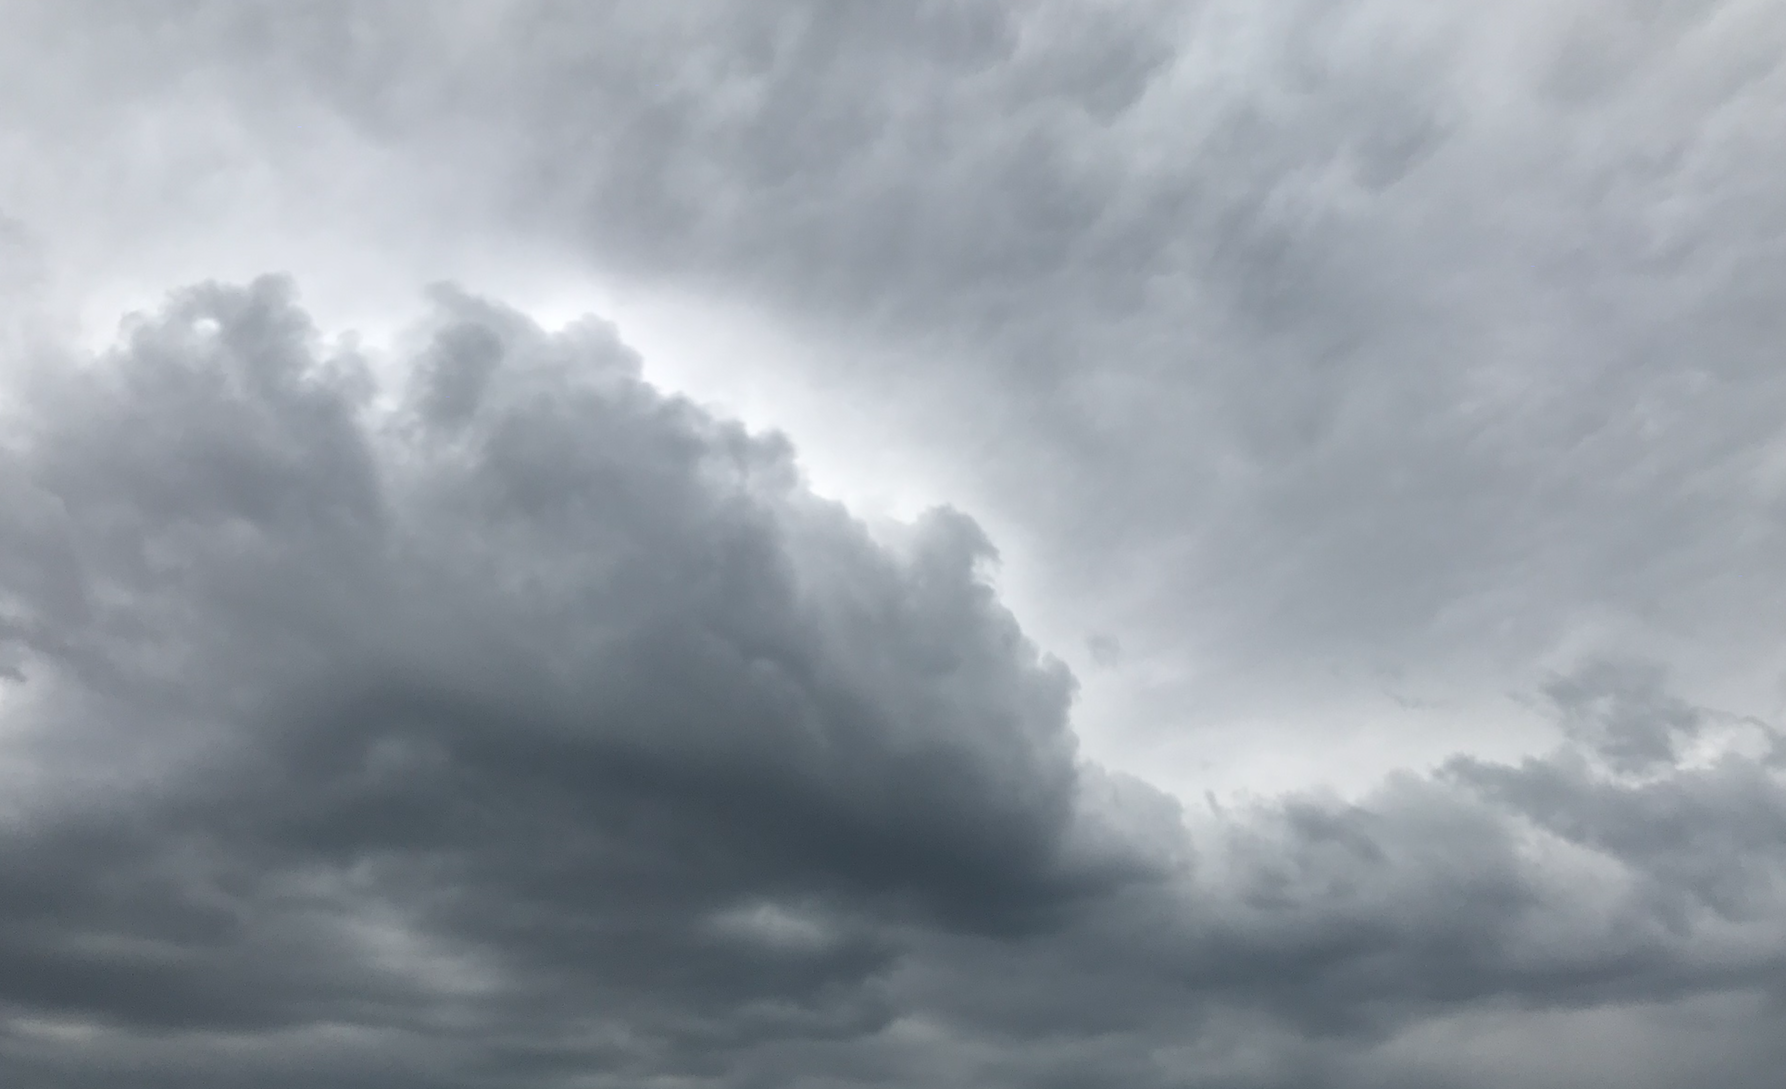
\includegraphics[width=\linewidth]{fig/photo/wetter.png}
    \captionof{figure}{Wetterverhältnisse am Tag der Messung (02.05.2019) }
	\label{fig:weather}
\end{center} 

Der Fit von \ch{O4} wurde im Channelbereich von $1500-1800$ ($461.76 - 489.80$\si{nm}) durchgeführt, wobei dieser Bereich bei einigen Messungen angepasst werden musste. 
Bei den Messungen 1, 4, 5 wurde ein Bereich von $466.58 - 485.26$ \si{nm} und bei Messung 2 ein Bereich von $466.58 - 482.52$ \si{nm} eingestellt.
Die Fitergebnisse sind in Tabelle \ref{fig:fit_multi_axis_DOAS} aufgetragen.
Eine $\Delta \text{SCD}$ Analyse der Daten erlaubt uns nun die oben erwähnte vertikale Verteilung der Gase zu untersuchen.

\begin{center}
	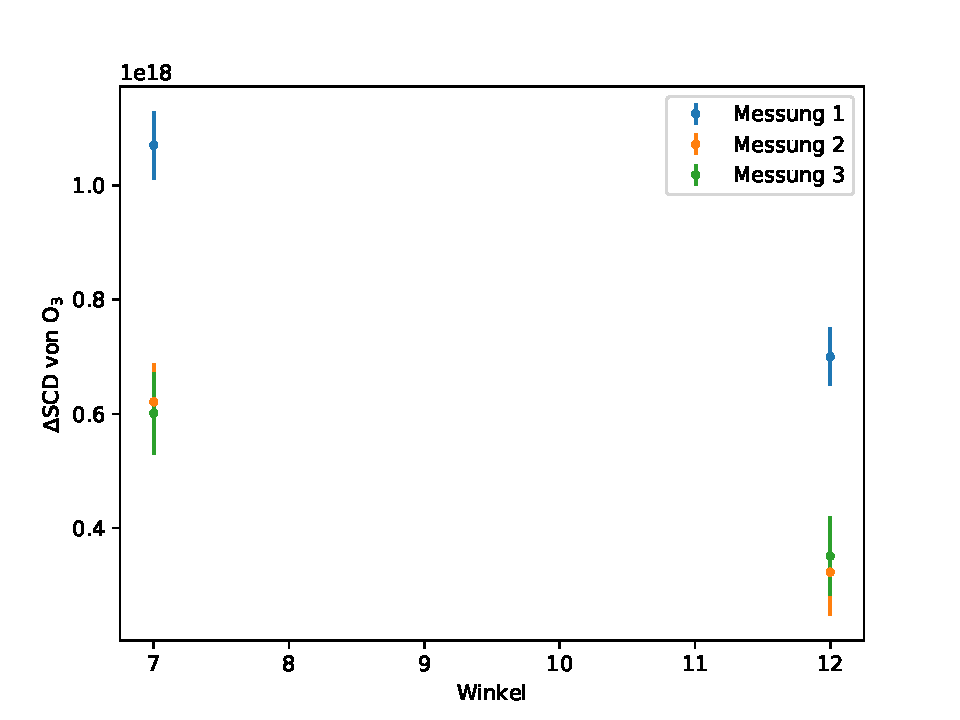
\includegraphics[width=\linewidth]{fig/max_DOAS_O3.pdf}
    \captionof{figure}{MAX-DOAS von \ch{O3}}
	\label{fig:max_doas_o3}
\end{center}

\begin{center}
	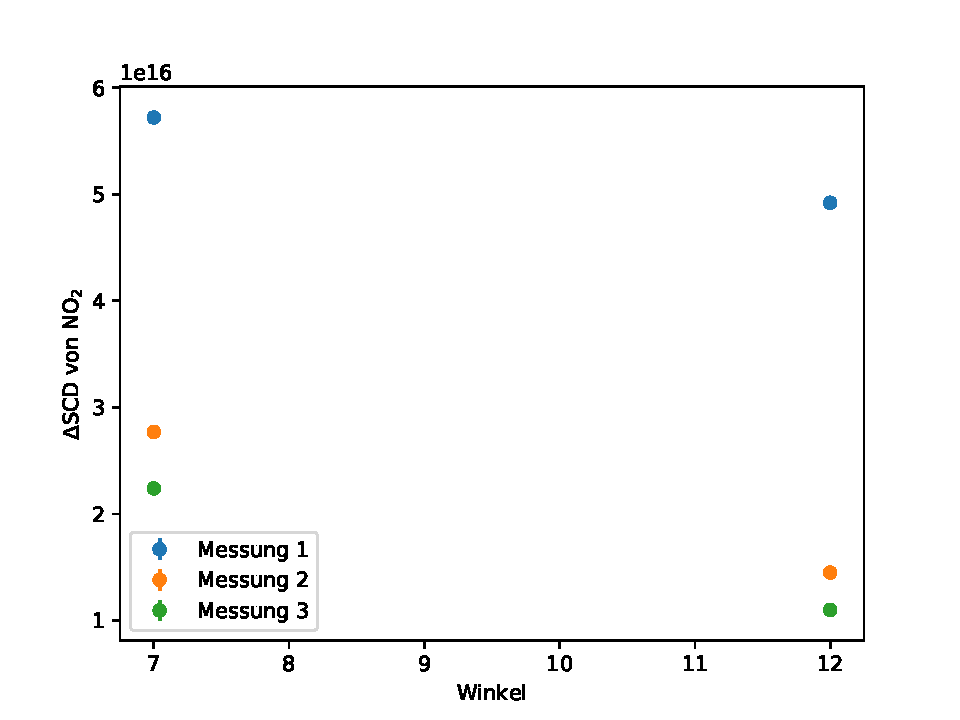
\includegraphics[width=\linewidth]{fig/max_DOAS_NO2.pdf}
    \captionof{figure}{MAX-DOAS von \ch{NO2}}
	\label{fig:max_doas_no2}
\end{center}

\begin{center}
	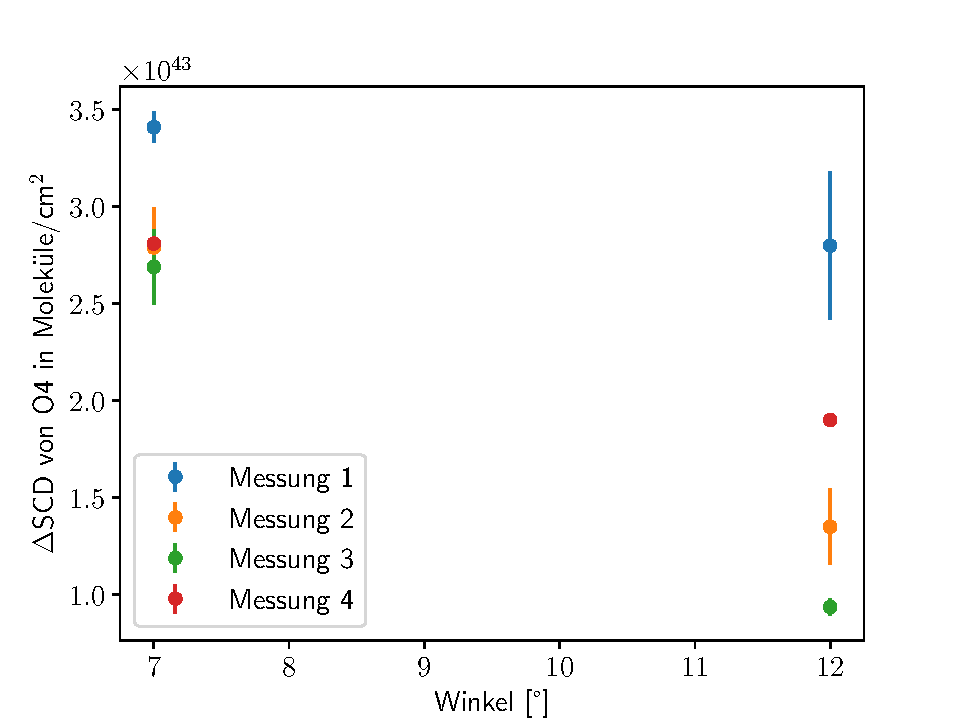
\includegraphics[width=\linewidth]{fig/max_DOAS_O4.pdf}
    \captionof{figure}{MAX-DOAS von \ch{O4}}
	\label{fig:max_doas_o4}
\end{center}

$\Delta$SCD gibt hierbei nur die Änderung von SCD in der Troposphäre an.
Dies kann man sehen, wenn man SCD als
\begin{align}
    \text{SCD} = \text{SCD}_\text{Trop} + \text{SCD}_\text{Strat},
\end{align}
schreibt.
Dann ist 
\begin{align}
\Delta\text{SCD} =& \text{SCD}_{\text{Mess}} - \text{SCD}_\text{ref} \\
    =& (\text{SCD}_{\text{Trop, \ Mess}} + \text{SCD}_{\text{Strat}}) \\
    & - (\text{SCD}_{\text{Trop, \ Ref}} + \text{SCD}_{\text{Strat}}) \\
    =& \text{SCD}_{\text{Trop, \ Mess}} - \text{SCD}_{\text{Trop, \ Ref}}. \label{eq:SCD_trop}
\end{align}

Über ein Vergleich der $\text{VCD}_{strat}$ (berechnet in Abschnitt \ref{sssec:tagesmessung})
und der hier bestimmbaren $\text{VCD}_{trop}$  von \ch{O3} kann darauf geschlossen werden, dass \ch{O3} hauptsächlich in der Stratosphäre gefunden werden kann.
Zur Berechnung von $\text{VCD}_{trop}$ müssen zunächst ein paar Vorüberlegungen angestrengt werden.
Zunächst gilt für den troposphärischen \textit{air mass factor}

\begin{align}
AMF_{trop}(\alpha) = \frac{SCD_{trop}(\alpha)}{VCD_{trop}},
\end{align}

was sich nun mit Gleichung \ref{eq:SCD_trop} zu 

\begin{align}
    VCD_{trop}(\alpha) = \frac{\Delta SCD_{trop}(\alpha)}{AMF_{trop}(\alpha)-AMF_{trop}(ref)}, 
\end{align} 

ergibt.
In unserem Fall ist es möglich den \textit{air mass factor} mit

\begin{align}
AMF_{trop} \approx \frac{1}{sin(\alpha)}
\end{align}

zu nähern, sodass sich schlussendlich die VCD bestimmen lässt.

\begin{align}
VCD_{trop} = \frac{\Delta SCD_{trop}(\alpha)}{\frac{1}{\sin(\alpha)}-1}.
\end{align}

Die Messungen von \ch{O3} ergeben nun VCD, die in der Tabelle aufgezeigt sind.

\begin{center}
	
	\begin{tabular*}{\linewidth}{c c c}
		\toprule
		Messung & Winkel & VCD [$\frac{\text{Moleküle}}{\si{cm}^2}$] \\
		\midrule
		1 & 7 & $1.51 \cdot 10^{17} \pm 8.19 \cdot 10^{15}$  \\
		& 12 & $2.00 \cdot 10^{17} \pm 1.34 \cdot 10^{16}$\\
		2 & 7 & $8.62 \cdot 10^{16} \pm 9.41 \cdot 10^{15}$ \\
		& 12 & $8.48 \cdot 10^{16} \pm 2.00 \cdot 10^{16}$\\
		3 & 7 &  $8.34 \cdot 10^{16} \pm 9.99 \cdot 10^{15}$\\
		& 12 & $9.21 \cdot 10^{16} \pm 1.82 \cdot 10^{16}$\\
		4 & 7 & $1.22 \cdot 10^{17} \pm 9.94 \cdot 10^{15}$ \\
		& 12 & $1.98 \cdot 10^{17} \pm 2.00 \cdot 10^{16}$\\
		\bottomrule
	\end{tabular*}
	\captionof{table}{$VCD_{trop}$ der verschiedenen \ch{O3} Messungen} 
	\label{fig:VCD_O3_trop}
\end{center}

Es wurden somit $VCD_{trop}$ Werte im Bereich von $3.3 - 7.7 \si{DU}$ gemessen. Dadurch lässt sich mit dem Vergleich zur stratosphärischen Messung von $\sim 300 \si{DU}$ (vgl. Abbildung \ref{fig:VCD_O3_over_day}) festhalten, dass \ch{O3} vorwiegend in der Stratosphäre vorkommt.\\

Einen qualitativen Ansatz liefert das Verhältnis der $\Delta$SCD Werte der $7°$ und $12°$ Messungen, da dies darüber Aufschluss gibt, welches Spurengas am stärksten von der Verlängerung der Weglänge in der Troposphäre abhängig ist. 	
Bei niedrigen Winkeln sind die Lichtstrahlen statistisch länger in der Troposphäre und werden daher stärker von dort vorkommenden Spurengasen absorbiert.
Den niedrigsten Wert hatte hier \ch{O3}, dies untermauert nun, dass es hauptsächlich in der Stratosphäre vorzufinden ist.
Im Gegensatz dazu hatte \ch{O4} die stärkste Veränderung. \\

\begin{center}
	
	\begin{tabular*}{\linewidth}{@{\extracolsep{\fill}} c c}
		\toprule
        Molekül & Verhältnis $\Delta \text{SCD}$ \\
        \midrule
        \ch{O3} & $1.0 \pm 0.4$ \\
        \ch{NO2} & $1.4 \pm 1.1$ \\
        \ch{O4} & $1.7 \pm 0.7$\\
		\bottomrule
	\end{tabular*}
    \captionof{table}{Verhältnis der $\Delta$SCD von \ch{O3}, \ch{NO2} und \ch{O4}} 
	\label{fig:ratio_dscd}
\end{center}

Am Tag der Messung war es sehr bewölkt, so dass man davon ausgehen kann dass $\Delta$VCD von \ch{O4} sehr stark von der Bewölkung abhängt.
Eine abschließende und genau Beurteilung der Messergebnisse ließen die Wetterverhältnisse nicht zu, da eine dichte Wolkendecke die Messergebnisse stark beeinflusste, die Messdaten legen nur die Vermutung nahe, dass \ch{O4} und \ch{NO2} auch vermehrt in der Troposhäre zu finden sind.


\section{Diskussion}\label{sec:discussion}

Der Versuch behandelt verschiedene Einsatzmöglichkeiten der DOAS Methode zur Bestimmung der atmosphärischen Spurengase.\\
 
Zu Beginn wurde die Messapparatur kennengelernt und auf mögliche systematische Fehler wie der Offset und Dunkelstrom untersucht, die beide jeweils einen linearen Zusammenhang mit der Anzahl der Scans aufwiesen. 
Im verwendeten Analyseprogramm \verb*+DOASIS+ wurden die Werte der beiden Einflüsse hinterlegt, um im Verlauf des Versuches die aufgenommenen Spektren korrigieren zu können. 
Des weiteren wurde auf Rauschen untersucht, dass im Verlauf des Versuchs über eine große Anzahl an Scans pro Spektrum jedoch minimiert wurde.
Eine Kalibrierung der Software \verb*+DOASIS+ wurde ebenfalls durchgeführt um in nachfolgenden Versuchsteilen sinnvolle Vergleichswerte für die Fitbereiche zu erhalten.\\

Eine erste Anwendung von DOAS wurde dann mit einer Labormessung der Konzentration von \ch{NO2} in einer Glasküvette kennengelernt. 
Dabei handelt es sich um eine \textit{aktive} DOAS Messung, da das Spektrometer direkt auf die Lichtquelle gerichtet wird. 
Über eine Anpassung des Fitbereichs auf die gut erkennbaren \ch{NO2} Strukturen konnte eine Konzentration von $(2.48 \pm 0.12) \cdot 10^{20} \Bigl[ \frac{\text{Moleküle}}{\ell}\Bigr]$, bzw. einem Mischungsverhältnis von $(9.311 \pm 0.004) \si{ppt}$ berechnet werden. 
Um diese Werte zu erhalten wurde die Fitroutine von \verb*+DOASIS+ verwendet, welche einen $\chi^2$ Wert von $4.367 \cdot 10^{-3}$ ermittelte. Auch über die erhaltenen Fitresiduals, welche sich im Größenordnungsbereich von $\pm 1 \cdot 10^{-2}$ bewegten, konnte nochmals die Qualität des Fits bestätigt werden.\\

Eine andere Einsatzmethode wurde im dritten Versuchsteil vorgestellt, wo vor allem die stratosphärische Konzentration von \ch{O3} und \ch{NO2} untersucht wurde.
Zunächst wurden die Messungen vom 23.04.2019 untersucht.
Das Teleskop wurde senkrecht in Himmel ausgerichtet, was dafür sorgt, dass hauptsächlich die stratosphärischen Konzentrationen aufgenommen wurden.
Hierbei wurde die SCD über den Tag bestimmt.
Interessant war hier, dass im \ch{NO2} Bild der Einfluss des Feierabendverkehrs beobachtet werden konnte.\\
Anschließend wurden Langley-Plots erstellt, mithilfe derer man die VCD bestimmen kann, falls die Langley-Plots linear sind.
Dies war für \ch{O3} der Fall.
Es zeigte sich, dass das VCA von \ch{O3} bei ca. 300\si{DU} lag.
Der Wert wurde mit Satellitenbildern verglichen, wobei sich zeigte, dass die Werte der Satelliten beide um ca 50 \si{DU} höher lagen.
Grund hierfür war, dass in der unsrigen Messung die troposphärische Konzentration nicht berücksichtigt wurde.\\

Im letzten Versuchsteil wurden jeweils vier Messungen bei $7^\circ$ und $12^\circ$ zwischen Kamera und Boden durchgeführt.
Dies gibt Ausschluss darüber welche Spurengase eher in der Troposphäre und welche eher in der Stratosphäre auftreten.
Hier lassen sich keine genauen Aussagen treffen, da die Daten nicht sehr eindeutig waren da der Himmel am Tag der Messung stark bewölkt war.
Allerdings lässt sich die Tendenz erahnen, dass \ch{O3} vor allem in der Stratosphäre auftritt. Für \ch{NO2} und \ch{O4} lässt sich eine höhere Abhängigkeit von dem Teleskopwinkel beobachten, sodass der Schluss nahe liegt, dass diese auch vermehrt in der Troposhäre zu finden sind.


\nocite{*}
\appendix
\end{multicols}
\newpage

% TABELLEN
\section{Tabellen}\label{tables}
\newcolumntype{d}[1]{D{.}{.}{3.1}}
\begin{center}
	
	\begin{tabular*}{\linewidth}{@{\extracolsep{\fill}} c d{1} c}
		\toprule
		Belichtungszeit [\si{ms}] & \multicolumn{1}{c}{Mittelwert [$\frac{\text{counts}}{\text{pixel}}$]} & Standardabweichung [$\frac{\text{counts}}{\text{pixel}}$] \\
		52500 & $316.0$ & $460.9$ \\
		45000 & $270.2$ & $401.9$ \\
		37500 & $223.9$ & $340.7$ \\
		30000 & $177.8$ & $277.0$ \\
		22500 & $132.1$ & $213.4$ \\
		15000 & $87.2$ & $155.6$ \\
		7500 &  $43.3$ & $105.9$ \\
		\bottomrule
	\end{tabular*}
	
	\captionof{table}{Dunkelstrom bei unterschiedlichen Belichtungszeiten} 
	\label{fig:dark_current_exposure_time}
\end{center}

%\vspace{2cm}
\vfill
\begin{center}
	
	\begin{tabular*}{\linewidth}{@{\extracolsep{\fill}} c c c}
		\toprule
		Anzahl der Scans & Mittelwert [$\frac{\text{counts}}{\text{pixel}}$] & Standardabweichung [$\frac{\text{counts}}{\text{pixel}}$] \\
		\midrule
		10000 & $-1112.8$ & $343.6$ \\
		8500 & $-1107.8$ & $315.9$ \\
		7000 & $-444.5$ & $281.4$ \\
		5500 & $109.1$ & $258.9$ \\
		4000 & $-147.9$ & $219.1$ \\
		2500 & $-188.7$ & $170.5$ \\
		1000 &  $-8.7$ & $109.6$ \\
		\bottomrule
	\end{tabular*}
	
	\captionof{table}{Differenz Offset bei unterschiedlicher Scanzahl} 
	\label{fig:difference_offset}
\end{center}

%\vspace{2cm}
\vfill
\begin{center}
	
	\begin{tabular*}{\linewidth}{@{\extracolsep{\fill}} c c c}
		\toprule
		Anzahl der Scans & Mittelwert [$\frac{\text{counts}}{\text{pixel}}\cdot 10^{-15}$] & Standardabweichung [$\frac{\text{counts}}{\text{pixel}}$] \\
		\midrule
		10000 & $47$ & $658.8$ \\
		8500 & $170$ & $538.3$ \\
		7000 & $29$ & $488.3$ \\
		5500 & $94$ & $443.0$ \\
		4000 & $-49$ & $371.2$ \\
		2500 & $-9.5$ & $299.0$ \\
		1000 &  $3.3$ & $190.1$ \\
		\bottomrule
	\end{tabular*}
	
	\captionof{table}{Differenz Offset bei unterschiedlicher Scanzahl (Halogen)} 
	\label{fig:difference_offset_halogen}
\end{center}

%\vspace{2cm}
\vfill

\begin{center}
	
	\begin{tabular*}{\linewidth}{@{\extracolsep{\fill}} c c c}
		\toprule
        Maximum & Wellenlänge \si{[nm]} & FWHM [\si{nm}] \\
		\midrule
		1 & $\sim 313$ & $1.2 \pm 0.1$ \\
		2 & $\sim 365$ & $0.8 \pm 0.1$ \\
		3 & $\sim 404$ & $0.6 \pm 0.1$ \\
		4 & $\sim 436$ & $0.7 \pm 0.1$ \\
		\bottomrule
	\end{tabular*}
	
	\captionof{table}{Optische Auflösung der verschiedenen Maxima} %\cite{atm_components}
	\label{fig:optical_resolution}
\end{center}

%\vspace{2cm}
\vfill

\begin{center}
	
	\begin{tabular*}{\linewidth}{@{\extracolsep{\fill}} c c c c c}
		\toprule
        Wellenlängenbereich \si{[nm]}&$\chi^{2}\cdot 10^{-4}$ & \multicolumn{1}{c}{Fit coeff. $\cdot 10^{15}$} & shift & squeeze \\
		\midrule
		$466.58 - 449.86$ & $8.67$ & $-484 \pm 1.97$ & $-0.00497 \pm 0.00495$ & $0.994 \pm 0.000333$ \\
		$413.46 - 449.74$ & $19.2$ & $-472 \pm 2.08$ & $0.0533 \pm 0.00682$ & $0.955 \pm 0.000261$\\
		$413.46 - 461.38$ & $33.2$ & $-475 \pm 2.23$ & $0.052 \pm 0.00682$ & $0.995 \pm 0.000246$ \\
		$413.46 - 477.25$ & $43.7$ & $-488 \pm 1.95$ & $0.091 \pm 0.00546$ & $0.993 \pm 0.000162$\\
		\bottomrule
    \end{tabular*}
	
	\captionof{table}{Fit bei verschiedenen  Fitbereichen}
	\label{fig:different_fit_ranges}
\end{center}

\vfill
\begin{center}
	
	\begin{tabular*}{\linewidth}{@{\extracolsep{\fill}} c c c c c}
		\hline %\toprule
		Molekül & Wellenlänge [\si{nm}] & Fit coeff. & shift & squeeze \\
		\hline %\midrule
		\ch{O3} & $311.07-339.71$ & $3.36 \cdot 10^{19} \pm 7.71 \cdot 10^{17}$ & $0.0135 \pm 0.00985$ & $0.992 \pm 0.00119$ \\
		\ch{NO2} & $413.40-467.43$ & $3.08 \cdot 10^{16} \pm 6.35 \cdot 10^{14}$ & $0.114 \pm 0.026$ & $0.99 \pm 0.000799$\\
		\ch{H2O} & $439.3-451.06$ & $7.68 \cdot 10^{21} \pm 1.19 \cdot 10^{22}$ & $0.0538 \pm 0.0264$ & $0.972 \pm 0.00372$ \\
		\ch{O4} & $440.13-451.57$ & $4.01 \cdot 10^{43} \pm 2.17 \cdot 10^{43}$ & $0.0439 \pm 0.0285$ & $0.972 \pm 0.00427$\\
		\hline %\bottomrule
	\end{tabular*}
	
	\captionof{table}{Fit mit Atmosphärendaten}
	\label{fig:fit_of_atmospheric_data}
\end{center}
\newpage
%\vspace{2cm}
\vfill
\begin{center}	
    %\hspace{-2em}
    %\begin{table}
        \begin{tabular}{@{\extracolsep{\fill}} c c c c c c}
		\hline %\toprule
		Nummer & Winkel & Molekül & Fit coeff. & shift & squeeze \\
		\hline %\midrule
		1 & 7 & \ch{O3} & $1.09 \cdot 10^{18} \pm 5.9 \cdot 10^{16}$ & $0.15 \pm 0.0227$ & $0.99 \pm 0.00244$ \\
		& & \ch{NO2} & $5.72 \cdot 10^{16} \pm 5.523 \cdot 10^{14}$ & $0.0716 \pm 0.0119$ & $0.993 \pm 0.000383$\\
		& & \ch{O4} & $3.41 \cdot 10^{43} \pm 8.08 \cdot 10^{41}$ & $0.308 \pm 0.0284$ & $0.988 \pm 0.00178$\\
		\cline{2-6}
		& 12 & \ch{O3} & $7.50 \cdot 10^{17} \pm 5.12 \cdot 10^{16}$ & $0.0213 \pm 0.0294$ & $1 \pm 0.00329$ \\
		& & \ch{NO2} & $4.92 \cdot 10^{16} \pm 5.39 \cdot 10^{14}$ & $0.0782 \pm 0.0144$ & $0.993 \pm 0.000463$\\
		& & \ch{O4} & $2.80 \cdot 10^{43} \pm 3.83 \cdot 10^{42}$ & $-0.699 \pm 0.0927$ & $1.02 \pm 0.00838$\\
		\hline
		2 & 7 & \ch{O3} & $6.21 \cdot 10^{17} \pm 6.78 \cdot 10^{16}$ & $0.028 \pm 0.0472$ & $1.01 \pm 0.00554$ \\
		& & \ch{NO2} & $2.77 \cdot 10^{16} \pm 6.31 \cdot 10^{14}$ & $0.0455 \pm 0.0296$ & $0.992 \pm 0.000949$\\
		& & \ch{O4} & $2.79 \cdot 10^{43} \pm 2.07 \cdot 10^{42}$ & $-0.331 \pm 0.0791$ & $1 \pm 0.00758$\\
		\cline{2-6}
		& 12 & \ch{O3} & $3.23 \cdot 10^{17} \pm 7.61 \cdot 10^{16}$ & $-0.489 \pm 0.0549$ & $1.05 \pm 0.00844$ \\
		& & \ch{NO2} & $1.45 \cdot 10^{16} \pm 6.10 \cdot 10^{14}$ & $0.0375 \pm 0.0549$ & $0.991 \pm 0.00176$\\
		& & \ch{O4} & $1.35 \cdot 10^{43} \pm 1.97 \cdot 10^{42}$ & $-0.314 \pm 0.151$ & $1.01 \pm 0.0149$\\
		\hline
		3 & 7 & \ch{O3} & $6.01 \cdot 10^{17} \pm 7.20 \cdot 10^{16}$ & $-0.0773 \pm 0.0515$ & $1.01 \pm 0.00596$ \\
		& & \ch{NO2} & $2.24 \cdot 10^{16} \pm 5.85 \cdot 10^{14}$ & $0.0582 \pm 0.034$ & $0.993 \pm 0.00109$\\
		& & \ch{O4} & $2.69 \cdot 10^{43} \pm 1.95 \cdot 10^{42}$ & $-0.32 \pm 0.0884$ & $0.998 \pm 0.00815$\\
		\cline{2-6}
		& 12 & \ch{O3} & $3.51 \cdot 10^{17} \pm 6.94 \cdot 10^{16}$ & $-0.106 \pm 0.0847$ & $1 \pm 0.00946$ \\
		& & \ch{NO2} & $1.10 \cdot 10^{16} \pm 5.37 \cdot 10^{14}$ & $-0.00289 \pm 0.0639$ & $0.994 \pm 0.00205$\\
		& & \ch{O4} & $9.36 \cdot 10^{42} \pm 4.43 \cdot 10^{41}$ & $-0.388 \pm 0.125$ & $1.01 \pm 0.00768$\\
		\hline
		4 & 7 & \ch{O3} & $8.81 \cdot 10^{17} \pm 7.16 \cdot 10^{16}$ & $0.361 \pm 0.0339$ & $0.977 \pm 0.00858$ \\
		& & \ch{NO2} & $2.6 \cdot 10^{16} \pm 5.13 \cdot 10^{14}$ & $0.0915 \pm 0.0268$ & $0.991 \pm 0.000906$\\
		& & \ch{O4} & $2.81 \cdot 10^{43} \pm 3.52 \cdot 10^{41}$ & $-0.31 \pm 0.0256$ & $0.989 \pm 0.00159$\\
		\cline{2-6}
		& 12 & \ch{O3} & $7.53 \cdot 10^{17} \pm 7.60 \cdot 10^{16}$ & $0.179 \pm 0.0425$ & $0.992 \pm 0.00463$ \\
		& & \ch{NO2} & $2.00 \cdot 10^{16} \pm 4.75 \cdot 10^{14}$ & $0.0706 \pm 0.0325$ & $0.992 \pm 0.0011$\\
		& & \ch{O4} & $1.9 \cdot 10^{43} \pm 3.361 \cdot 10^{41}$ & $-0.209 \pm 0.0285$ & $0.981 \pm 0.00182$\\
        \hline %\bottomrule
	\end{tabular}
	
	\captionof{table}{Fitergebnisse verschiedener Winkel}
	\label{fig:fit_multi_axis_DOAS}
\end{center}

\newpage
\printbibliography

\end{document}

